\documentclass{article}
\usepackage{graphicx} % Required for inserting images
\usepackage{booktabs}
\usepackage{microtype}
\setlength{\emergencystretch}{1.5em}
\usepackage{array}
\newcolumntype{L}[1]{>{\raggedright\arraybackslash}p{#1}}
\usepackage{amsmath}
\usepackage[hyphens]{url}
\usepackage{tikz}
\usetikzlibrary{arrows.meta,positioning,shapes.symbols}
\usepackage{placeins}
\usepackage{pdflscape}

\title{Compiling Snort~3 Rule Headers into Conservative P4 Prefilters: An Evaluation on BMv2}
\author{
  Arthur de Freitas Medeiros\\
  Universidade Federal do Pampa (UNIPAMPA)\\
  Alegrete, Brazil\\
  \texttt{arthurfreitas.aluno@unipampa.edu.br}
}
\date{October 2026}

\begin{document}

\maketitle

\begin{abstract}
Programmable data planes can evaluate lightweight packet predicates before a
software intrusion detection system (IDS), but Snort~3 rules also depend on
payload, stream, flow/state, and other semantics that a P4 target cannot
necessarily represent. We present a semantics-aware, target-aware
Snort-to-P4 compilation approach that classifies each rule-to-predicate
relation as \textsc{Exact}, \textsc{Necessary}, or \textsc{Unsupported}.
A necessary predicate is meant to retain every packet satisfying its source
rule within an explicitly enforced packet domain, while omitted semantics
remain explicit in a manifest recording predicate-to-rule provenance.
Packets outside that domain, such as those carrying IPv4 options, fragments,
or truncated headers, are failed open as conservative candidates instead of
being matched against fields the parser cannot locate. What a header
condition guarantees depends on how the IDS evaluates it: once Snort~3
identifies a flow's service, it ignores the header ports and protocol of
service-based rules, so the compiler keeps only their addresses. An earlier
compilation that kept those conditions over-constrained 2,931 predicates,
and one of its plans marked no-match, on BMv2, the witnesses of 190 HTTP
rules on which Snort alerted off their header port. Under the corrected
compilation, 3,996 of 4,017 rules are classified as necessary, 21 as
unsupported, and none as exact, and backend lowering produces 235 P4
entries. The global binary prefilter marked 100\% of parser-eligible packets
as candidates on SQLi, XSS, and held-out Brute Force traces replayed on BMv2,
and a strong-discriminator ablation that removes the broadest entries still
marked 92.2--94.9\%. Provenance supports an offline utility, per-packet
candidate rule sets, which average about four of the 739 rules that ablation
keeps P4-eligible; the 3,278 rules left in fallback apply to every packet,
however, and the held-out reduction over the full ruleset is 18.3\%, against
81.8\% under the earlier compilation. Observed alerts were preserved in the traces,
and in an end-to-end campaign over 1,000 sampled rules, with Snort~3 as the
oracle and BMv2 as the target, no rule that a plan prefilters alerted on a
witness the data plane marked no-match. These results show that semantic
safety and operational selectivity are distinct, and that much of the
selectivity a header-derived prefilter appears to offer can come from
conditions the IDS does not check; candidate-set-aware IDS execution remains
future work.
\end{abstract}

\section{Introduction}
Signature-based network IDSs remain dependent on rules that combine packet
headers with payload inspection, stream and flow state, service semantics,
and temporal conditions. These conditions cannot generally all be represented
by a programmable data-plane target. The resulting challenge is not merely
to translate rule syntax to P4, but to partially compile Snort 3 detection
semantics without obscuring what the target cannot represent.

Programmable data planes can evaluate lightweight packet predicates before
software IDS processing. Prior P4-based IDS and prefiltering efforts motivate
this form of data-plane assistance \cite{lewis2019p4id,tavares2021p4onids},
while work on rule-based prefiltering emphasizes the importance of retaining
the context required by the IDS \cite{brum2025rethinking}. However, the
interaction between semantic preservation, target limitations, and
ruleset-scale selectivity remains insufficiently characterized.

A Snort rule may contain representable header predicates together with
payload, stream, flow/state, normalization, or service-dependent conditions.
Compiling only the representable subset without recording the omitted
semantics risks presenting a partial implementation as equivalent to the
original rule. A safe necessary prefilter instead establishes, for a rule
$r$ and generated predicate $p_r$, the relation $r \Rightarrow p_r$ under a
stated semantic profile and a stated packet domain; it does not assume
$p_r \Rightarrow r$ or $r \Leftrightarrow p_r$. Traffic the data plane
cannot parse as intended is retained by failing open rather than being
matched against fields read from the wrong offset. The detailed model is
developed in the problem formulation.

Semantic safety alone, however, does not determine operational usefulness.
When thousands of necessary predicates are aggregated into a global binary
candidate decision, their union can cover nearly all traffic in a workload.
Semantic coverage and packet-level selectivity must therefore be evaluated as
separate properties. Moreover, the binary decision discards which predicate
and which source rule produced a match. Retaining predicate provenance enables
an alternative question: not only whether a packet remains a candidate for
IDS handling, but which IDS rules remain plausible candidates for that packet.
This is evaluated here as an offline candidate-rule-space opportunity, not as
an implemented runtime execution mechanism.

This paper develops and evaluates a semantics-aware, target-aware compilation
workflow from Snort 3 rules to P4 predicates, with explicit delegation and
fallback. Under the evaluated configuration, 3,996 of 4,017 rules admitted
necessary predicates. For the 2,931 service-based rules among them, those
predicates keep only the header addresses, because Snort~3 stops checking
ports and protocol once it identifies the flow's service; an earlier
compilation that kept them is reported for what it missed. The global
binary prefilter marked 100\% of parser-eligible packets as candidates in
the three evaluated traces. Provenance-based analysis reduced the mean
per-packet candidate set by more than 99\% within the 739 rules that a
strong-discriminator ablation keeps P4-eligible, but by only 18.29--18.30\%
over the full ruleset; under the earlier compilation the held-out reduction
over the full ruleset was 81.81\%. These
observations motivate the following contributions and research questions.

\subsection{Contributions}
This work makes the following contributions:
\begin{itemize}
    \item A semantics-aware, target-aware method for deriving P4-executable
    predicates from Snort 3 rules and classifying their relation as
    \textsc{Exact}, \textsc{Necessary}, or \textsc{Unsupported}.
    \item A compilation manifest that records preserved and delegated
    predicates, fallback and unsupported rules, and provenance linking final
    P4 entries to source Snort rule identifiers.
    \item A P4 backend that performs predicate expansion, normalization,
    target-aware lowering, deduplication, and P4Runtime installation-plan
    generation; the evaluated backend reduces 4,040 predicate instances to
    235 final installation entries as installation state.
    \item An explicitly enforced packet domain that gates predicate
    evaluation on IPv4 header form and fails open for options, fragments,
    truncated headers, and parser errors, validated by a controlled
    data-plane suite and by trace-level replay accounting.
    \item An empirical evaluation that separates semantic safety from
    ruleset-scale packet-level selectivity, including a causal analysis of
    broad predicates and distributed union coverage.
    \item A provenance-based, offline candidate-rule-space analysis, which
    reduces the mean per-packet candidate set by more than 99\% within the
    P4-eligible partition but by at most 18.40\% over the full ruleset, and a
    measurement of the candidate set that a grouped prefilter would forward.
    \item An analysis, from the Snort~3.12.2.0 source, showing that
    service-based rules, whether they declare a \texttt{service} option or
    acquire a service through their options, do not make their header ports
    and protocol necessary conditions; a compilation that follows this rule
    for the 2,931 affected rules; and a measurement, on BMv2 and over the
    traces, of what an earlier compilation that kept those conditions missed
    and of the selectivity it had appeared to offer.
    \item Empirical validation of semantic-split behavior and observed P4
    alert-packet preservation, without claiming formal equivalence or dynamic
    stateful candidate-set execution.
    \item An end-to-end differential campaign that synthesizes a witness flow
    per rule and compares Snort~3 alerts with BMv2 verdicts frame by frame,
    observing no violation over a stratified sample of 1,000 rules under
    either plan and measuring how much the evaluated plans can falsify.
\end{itemize}

\subsection{Research Questions}
\textbf{RQ1 -- Semantic Coverage.} To what extent can Snort 3 rules be
safely represented by predicates executable in a programmable P4 data
plane while explicitly preserving semantic limitations?

\textbf{RQ2 -- Backend Feasibility.} Can the semantically derived
predicates be lowered and installed in a practical P4 target without
hiding unsupported semantics or exceeding target constraints?

\textbf{RQ3 -- Operational Selectivity.} How selective is a binary P4
prefilter when thousands of semantically safe predicates are jointly deployed?

\textbf{RQ4 -- Detection Preservation and Alternative Utility.} When
packet-level bypass selectivity is limited, can the compiled predicates
still preserve observed IDS alerts and reduce the per-packet candidate
rule space?

\subsection{Paper Organization}
The remainder of the paper presents background and related work, followed by
the problem formulation and proposed approach. It then describes the
experimental methodology, results, discussion, threats to validity and
limitations, conclusion, and the experimental-profile appendix.

\section{Background}
\label{sec:background}
\subsection{Snort 3 Rule Semantics}
Snort \cite{roesch1999snort} is a signature-based network IDS; this work
targets Snort~3 \cite{snort3manual}. A Snort~3 text rule has a header and a
body. The header names an action, a protocol, the source address and port, a
direction that is either unidirectional or bidirectional (\texttt{<>}), and
the destination address and port; addresses and ports may be variables such
as \texttt{\$HOME\_NET} or the wildcard \texttt{any}. The body, in
parentheses, holds options: payload options such as \texttt{content} and
\texttt{pcre} that inspect a buffer, flow options such as \texttt{flow} and
\texttt{flowbits} that depend on session state, and metadata such as
\texttt{sid}. Snort selects candidate rules with a fast-pattern search and
then evaluates each candidate's options left to right, stopping at the first
one that fails.

Snort~3 also distinguishes port-based from service-based rules. A rule is
service-based when it declares a \texttt{service} option, uses an option
specific to a service, or names a service protocol in its header, as in
\texttt{alert http}. Every header component of a port-based rule must match.
Once Snort has identified the flow's service as one of the services of a
service-based rule, it checks the rule's header addresses but not its ports
or protocol; a rule that names the service protocol in its
header keeps its port checks (Section~\ref{sec:service-based}). A header predicate taken from a rule is
therefore an approximation whose relation to the rule has to be stated rather
than assumed.

\subsection{P4 Programmable Data Planes}
P4 \cite{bosshart2014p4} programs describe how a data plane parses packets and
processes them through match-action tables; this work uses
P4$_{16}$ \cite{p4spec2023}. A parser extracts headers into typed fields, and
control blocks apply tables whose keys use match kinds such as
\texttt{exact}, \texttt{ternary}, and \texttt{lpm}; the v1model architecture
adds \texttt{range} and \texttt{optional}. The program fixes which fields a
table can match, while the control plane installs the entries at run time.
The evaluated target is BMv2 \cite{bmv2}, whose \texttt{simple\_switch\_grpc}
process implements the v1model architecture and serves the P4Runtime
API \cite{p4runtime2024}. Through it a controller installs the pipeline
configuration and writes table entries, and ternary entries carry a priority
that orders overlapping matches. The evaluated backend uses target-supported
Ethernet/IPv4 header fields as a candidate marker; it does not replace Snort
detection.

\subsection{Semantic Preservation and Prefiltering}
Necessary predicates can safely retain traffic for Snort inspection, but
their joint deployment need not provide useful packet-bypass selectivity.

\section{Related Work}
\label{sec:related}
\subsection{Rule-Derived and Hybrid P4 IDS Offloading}
Rule-derived filtering has established that programmable data planes can
assist software IDS processing. P4ID \cite{lewis2019p4id} derives packet
filters from Snort rules using information such as IP addresses,
transport-layer ports, protocols, and TCP flags, and combines stateless and
stateful packet-processing stages. It therefore demonstrates both
rule-derived filtering and stateful data-plane assistance. P4-ONIDS
\cite{tavares2021p4onids} addresses constrained data planes through range
representation, rule aggregation, deduplication, and flow information to
limit packets forwarded to the NIDS.

4MIDable \cite{lewis2023fourmidable} provides a framework for integrating
existing security middleboxes with P4/SDN infrastructure. Its P4ID agent
supports stateful processing and feedback to an unmodified IDS, and was
evaluated on both software BMv2 and hardware Tofino targets. The work reports
traffic-processing reductions without affecting observed detection rates.
P4NIPS \cite{senoski2025p4nips} provides a recent P4 network-intrusion
prevention implementation. Together, these systems show the feasibility of
rule-derived filtering, hybrid IDS/data-plane integration, stateful
assistance, and resource-aware P4 representations; they are not treated here
as evidence for a common per-rule semantic relation between a source IDS rule
and a generated predicate.

\subsection{Context Preservation and Hybrid IDS Processing}
Brum et al. \cite{brum2025rethinking} revisit rule-based NIDS
pre-filtering by considering traffic required for subsequent IDS processing
even when a packet does not directly satisfy extracted rule conditions. Their
eRBF approach incorporates flow context, including TCP connection
establishment and termination information and selected protocol dependencies.
Evaluated with Snort~3 and large rulesets, it shows why aggressive
pre-filtering must account for context required by the IDS. Its software
trace-based evaluation, however, does not address the mapping of those
semantics to a P4 target's processing and resource constraints.

RNA \cite{hagen2025rna} follows a complementary event-oriented direction:
it analyzes selected Zeek-script events and maps them to protocol and event
templates for programmable forwarding devices, together with complementary
host-side mechanisms. This coordinated generation illustrates how selected
IDS functionality can be distributed across host and data-plane components.
Its scope is selected Zeek events and predefined templates rather than a
general semantic classification of signature-based IDS rules according to the
guarantees preserved by their data-plane representation.

\subsection{Programmable-Data-Plane Security Landscape}
The broader programmable-data-plane literature situates IDS offloading among
other security applications and target models. Surveys of P4 fundamentals and
applications \cite{hauser2023p4survey}, P4 security applications and their
vulnerability context \cite{alsabeh2022p4securitysurvey}, and
programmable-data-plane IDS approaches \cite{fida2026pdpids} document the
breadth of the field. Implementation-oriented work also emphasizes that
mapping security functionality to programmable targets involves resource and
implementation constraints \cite{mazloum2025p4security}. These sources
motivate target-aware treatment of security functionality; they do not by
themselves establish properties of the individual systems compared above.

\subsection{Positioning of This Work}
Prior systems demonstrate that rule-derived filtering, stateful assistance,
resource-aware P4 representations, and coordinated IDS/data-plane execution
are feasible. This work focuses on making the semantic consequences of
partial compilation explicit. It classifies the relation between each source
Snort rule and generated P4 predicate, records preservation, delegation, and
fallback in a compilation manifest, and retains source-rule provenance through
backend lowering and deduplication.

The evaluation also separates semantic safety from aggregate operational
selectivity: a safe necessary predicate can be retained for Snort inspection
yet contribute to a global binary candidate union that is not selective.
Rather than presenting that outcome as a successful traffic-bypass result,
the analysis uses retained provenance to examine an offline per-packet
candidate-rule-space opportunity. Thus, the contribution is not Snort-to-P4
translation alone, but explicit semantic and target-aware characterization of
what is preserved, delegated, and still operationally useful.
Table~\ref{tab:related-work-comparison} compares these dimensions across the
reviewed work.

\begin{landscape}
\begin{table}[p]
\centering
\small
\setlength{\tabcolsep}{2pt}
\renewcommand{\arraystretch}{0.95}
\caption{Related-work comparison. ``Not explicit'' denotes information not
established in the reviewed scope, rather than absence of the feature.}
\label{tab:related-work-comparison}
\begin{tabular}{L{1.45cm}L{2.20cm}L{1.90cm}L{2.00cm}L{2.35cm}L{2.80cm}L{2.20cm}L{3.25cm}}
\toprule
\textbf{Work} & \textbf{Source IDS / rules} & \textbf{P4 target} & \textbf{Rule-derived filtering} & \textbf{State / context handling} & \textbf{Explicit semantic relation} & \textbf{Provenance retained} & \textbf{Main objective} \\
\midrule
P4ID & Snort rules & P4 data plane & Yes & Yes (stateful stage) & Not explicit in reviewed scope & Not explicit in reviewed scope & Rule-derived IDS filtering \\
P4-ONIDS & NIDS rules & P4 data plane & Yes & Partial (flow information) & Not explicit in reviewed scope & Not explicit in reviewed scope & Resource-aware NIDS pre-filtering \\
4MIDable & Existing security middleboxes / P4ID agent & BMv2; Tofino & Yes & Yes & Not explicit in reviewed scope & Not explicit in reviewed scope & Hybrid security-VNF offloading \\
eRBF & Snort~3 rules & N/A (software trace model) & Yes & Yes & Not explicit in reviewed scope & Not explicit in reviewed scope & Context-preserving NIDS pre-filtering \\
RNA & Zeek events & P4 device + host & N/A & Partial (event / host coordination) & Not explicit in reviewed scope & Not explicit in reviewed scope & Event offload \\
P4NIPS & Not explicit in reviewed scope & P4 & Not explicit in reviewed scope & Not explicit in reviewed scope & Not explicit in reviewed scope & Not explicit in reviewed scope & NIPS implementation \\
This work & Snort~3 rules & BMv2 & Yes & Delegated to Snort & Yes (three classes) & Yes & Semantic transparency and selectivity analysis \\
\bottomrule
\end{tabular}
\end{table}
\end{landscape}

\section{Problem Formulation}
\label{sec:problem}
\subsection{Snort Rule Model}
A signature-based IDS rule can combine multiple conditions that depend
on different types of information. Some conditions can be evaluated
directly from packet headers, while others may depend on payload
contents, flow state, temporal relationships, protocol normalization,
or information collected across multiple packets. Therefore, a rule
cannot generally be treated as a single match-action entry when
considering its execution in a programmable data plane.

For the purposes of this work, a rule $r$ is represented as:
\[
r = (H_r, P_r, F_r, T_r, N_r, a_r, m_r),
\]
where $H_r$ represents header predicates, $P_r$ payload-dependent
predicates, $F_r$ flow and state conditions, $T_r$ temporal conditions,
$N_r$ normalization or protocol-dependent conditions, $a_r$ the
associated action, and $m_r$ rule metadata such as its identifier and
priority.
Given a target data plane $s$, only a subset of the predicates that
compose a rule may be executable by that target. We denote by $C_s$
the set of capabilities exposed by the target, such as exact, ternary,
or range matching over selected packet-header fields. The compilation
process analyzes each rule predicate with respect to $C_s$ and produces
a data-plane predicate $p_r$ together with a semantic classification.

\subsection{P4 Predicate Model and Semantic Relations}
In this initial model, the generated representation is assigned to one
of three classes:

\begin{itemize}
    \item \textbf{EXACT}: all predicates considered by the supported
    rule profile are represented without semantic relaxation in the
    generated data-plane predicate.

    \item \textbf{NECESSARY}: the generated predicate preserves only
    conditions that are necessary for the original rule to match.
    Therefore, packets that satisfy the generated predicate still
    require inspection by the original IDS.

    \item \textbf{UNSUPPORTED}: the compiler cannot derive a safe
    data-plane predicate under the capabilities assumed for the target,
    and evaluation remains delegated to the IDS.
\end{itemize}

\subsection{Safety Condition}
The semantic classification determines how the generated component can
be interpreted. An EXACT representation records no delegated, fallback, or
unassessed detection predicate within the supported profile. The current P4
program nevertheless implements candidate marking through the single
\texttt{send\_to\_ids} action rather than a general data-plane detection
action. A NECESSARY representation is used only as a conservative pre-filter: matching
traffic remains subject to inspection by Snort, since the data-plane
predicate alone is insufficient to reproduce the complete detection
decision. An UNSUPPORTED rule remains delegated to Snort. Therefore,
the existence of a data-plane match is not treated as equivalent to an
IDS alert unless the required semantic guarantees are satisfied.
For a rule $r$ and a generated NECESSARY predicate $p_r$, the safety
relation is $r \Rightarrow p_r$; the converse $p_r \Rightarrow r$ is not
assumed. UNSUPPORTED means that no safe selective P4 predicate was
established under the target profile, not that the rule is ignored.

\subsection{Predicate-Level Soundness of Partial Compilation}
The NECESSARY claim is a predicate-level statement under the current
Ethernet/IPv4 target profile, not a general claim about arbitrary Snort
execution. For a parsed rule $r$, let $H_r$ denote the conjunction of its
header conditions that the capability analysis marks \textsc{Preserved} or
\textsc{Expanded}; let $U_r$ denote the remaining detection-relevant
conditions recorded as delegated, fallback, or unassessed. A source-rule
match entails every header condition that Snort checks for that rule, and
the compiler restricts $H_r$ to those conditions, so that
$r(x) \Rightarrow H_r(x)$; Section~\ref{sec:service-based} identifies them
for the rules whose header Snort does not evaluate in full. The backend materializes a predicate $p_r=L(H_r)$ only for a prefilter
candidate. Under the implementation assumptions that the accepted header
forms are parsed and normalized as recorded in the manifest, and that lowering
does not exclude a packet satisfying $H_r$, the construction gives

\[
r(x) \Rightarrow H_r(x) \Rightarrow L(H_r)(x) = p_r(x).
\]

The implication uses no claim about the omitted $U_r$ conditions: their
presence can make $p_r$ broader, which is why NECESSARY is not EXACT. If the
compiler cannot establish a selective $H_r$, it emits no prefilter entry and
classifies the rule as UNSUPPORTED. EXACT would additionally require that all
detection-relevant predicates be represented without relaxation; no such rule
occurred in the evaluated Community ruleset.

\subsection{Service-Based Rules}
\label{sec:service-based}
The premise $r(x) \Rightarrow H_r(x)$ holds when Snort evaluates the whole
rule header, and Snort~3 does not always do so. In Snort~3.12.2.0, before the
header of a rule with services is checked, Snort compares the service it has
identified for the flow with the rule's services. If the identified service is
one of them, the port checks are skipped and the protocol check succeeds
unconditionally, while the address checks still run; if a different service
has been identified, the rule is rejected; only when no service has been
identified is the whole header checked (\path{src/detection/detection_options.cc}
and \path{src/detection/rtn_checks.cc} in the Snort~3.12.2.0 source). Snort's
documentation states a coarser form of this rule: for a service-based rule,
evaluation of the header is skipped \cite{snort3manual}. Service
identification can come from content inspection, so an HTTP request on a port
outside \texttt{HTTP\_PORTS} is still evaluated against the HTTP rules. One
form is an exception. A rule that names a service protocol in its header, such
as the twelve rules of the form \texttt{alert http} \dots\ \texttt{->} \dots\
in the evaluated ruleset, is marked as a user-mode rule when Snort builds its
header checks, and that restores the port checks
(\path{src/parser/parse_rule.cc} and \path{src/detection/fp_detect.cc}).

A rule need not declare its services. When the rules are loaded, an option
that selects a buffer registered by a service inspector adds that
inspector's services to a rule that has none, and a few option-name prefixes
add a guessed service (\path{src/detection/fp_utils.cc}). The DCE options
\texttt{dce\_iface} and \texttt{dce\_stub\_data}, for instance, add
\texttt{dcerpc} and \texttt{netbios-ssn}.

For a service-based rule whose header names an IP protocol, the header
condition that is necessary for an alert is therefore
$H_r^{\mathrm{addr}}$, the address part of its header; the full header is
necessary only for packets whose service Snort has not identified. The
compiler therefore represents these rules by $H_r^{\mathrm{addr}}$ and
delegates their ports and protocol to Snort. It keeps the protocol only when
the rule's \texttt{flags} option already restricts it to TCP, since that
option matches no other protocol. From here on, \emph{service-based} refers
to these rules only; the user-mode rules keep their port checks and are
compiled, like port-based rules, with their full header. An earlier version
of the compiler represented every rule by its full header;
Section~\ref{sec:service-exposure} measures how many rules that affected and
what it changed.

\subsection{Enforced Packet Domain}
\label{sec:packet-domain}
The implication above presupposes that the data plane reads the fields the
predicate refers to. That presupposition is not free: a parser that assumed a
fixed 20-byte IPv4 header would read IPv4 option bytes as transport ports, so
a packet satisfying $r$ could fail $p_r$ and the necessary relation would not
hold. The implementation therefore makes the precondition explicit rather
than assumed.

Let $D$ denote the \emph{supported packet domain}: untagged Ethernet carrying
direct IPv4 with $\mathrm{version}=4$, $\mathrm{IHL}=5$,
$\mathrm{fragOffset}=0$, flags either zero or \texttt{DF}, and no parser
error. The P4 parser gates L4 extraction on membership in $D$, and the
ingress control re-checks the same conditions before applying the predicate
table. For $x \notin D$, the pipeline executes
\texttt{packet\_domain\_fallback}, which marks the packet as a candidate
unconditionally and counts it on a dedicated index. Writing
$\mathrm{cand}(x)$ for the candidate outcome of the deployed pipeline:

\[
r(x) \Rightarrow
\begin{cases}
p_r(x) \Rightarrow \mathrm{cand}(x), & x \in D,\\
\mathrm{cand}(x), & x \notin D.
\end{cases}
\]

Consequently, no packet satisfying the rule is excluded from Snort
inspection, whether or not the parser can interpret it. The data plane fails
open by construction: a no-match verdict is emitted only inside $D$, because
no-match is the only outcome that could ever motivate bypassing the IDS.
This makes the domain a stated precondition of the selectivity metrics rather
than a hidden assumption, and it is why candidate rates in
Section~\ref{sec:results} are reported over $D$ with domain fallback counted
separately.

\subsection{Semantic Safety versus Operational Selectivity}
A predicate can be semantically safe as a necessary condition while still
matching most packets once it is jointly deployed with thousands of other
predicates. This distinction is evaluated explicitly in the results.
\section{Proposed Approach}
\label{sec:approach}
The proposed approach introduces a semantics-aware compilation pipeline
between Snort 3 rules and a programmable data plane. Instead of directly
converting a complete rule into P4 code, the pipeline first parses and
decomposes the rule into an intermediate representation. Each predicate
is then analyzed according to the capabilities of the selected P4 target.
The result of this analysis determines which components can be represented
in the data plane and which must remain delegated to Snort.

The proposed pipeline consists of five main stages: (i) Snort rule
parsing, (ii) construction of an intermediate representation,
(iii) target capability analysis, (iv) semantic classification, and
(v) generation of the corresponding data-plane configuration or IDS
fallback. Figure~\ref{fig:pipeline-architecture} places these stages
between their inputs and the BMv2 target.

\begin{figure}[t]
\centering
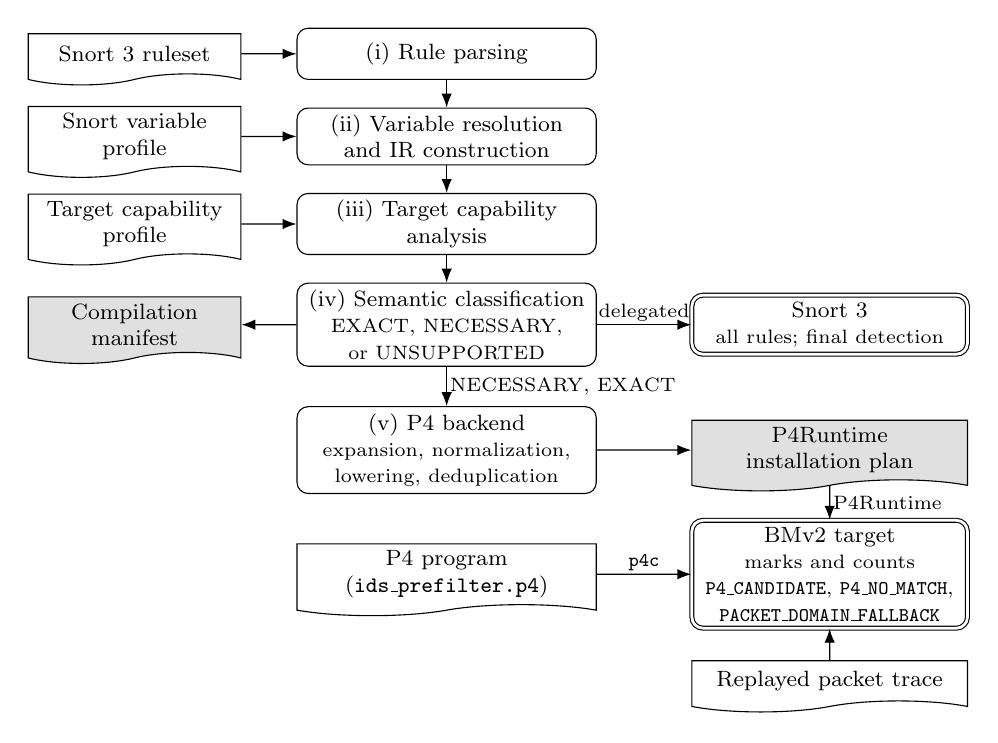
\begin{tikzpicture}[
  >=Latex,
  font=\footnotesize,
  stage/.style={draw, rounded corners, align=center, minimum width=38mm,
    minimum height=6.5mm, inner sep=2.5pt},
  artifact/.style={draw, shape=tape, tape bend top=none,
    tape bend height=1.4mm, align=center, minimum width=27mm,
    minimum height=6.5mm, inner sep=2.5pt},
  input/.style={artifact},
  output/.style={artifact, fill=black!12},
  target/.style={draw, double, double distance=1pt, rounded corners,
    align=center, minimum width=35mm, minimum height=6.5mm, inner sep=2.5pt},
  flow/.style={->, line width=.45pt},
  note/.style={font=\scriptsize, inner sep=1pt}
]
  % Compiler stages (center column)
  \node[stage] (parse) {(i) Rule parsing};
  \node[stage, below=3.5mm of parse] (ir)
    {(ii) Variable resolution\\and IR construction};
  \node[stage, below=3.5mm of ir] (cap)
    {(iii) Target capability\\analysis};
  \node[stage, below=3.5mm of cap] (cls) {(iv) Semantic classification\\
    {\scriptsize EXACT, NECESSARY,}\\{\scriptsize or UNSUPPORTED}};
  \node[stage, below=5mm of cls] (backend) {(v) P4 backend\\
    {\scriptsize expansion, normalization,}\\
    {\scriptsize lowering, deduplication}};

  % Inputs and manifest (left column)
  \node[input, left=7mm of parse] (rules) {Snort 3 ruleset};
  \node[input, left=7mm of ir] (vars) {Snort variable\\profile};
  \node[input, left=7mm of cap] (capprof) {Target capability\\profile};
  \node[output, left=7mm of cls] (manifest) {Compilation\\manifest};

  % Snort and data plane (right column)
  \node[output, minimum width=35mm, right=12mm of backend] (plan)
    {P4Runtime\\installation plan};
  \node[target] (snort) at (plan |- cls)
    {Snort 3\\{\scriptsize all rules; final detection}};
  \node[target, below=5mm of plan] (bmv2) {BMv2 target\\
    {\scriptsize marks and counts}\\
    {\scriptsize\texttt{P4\_CANDIDATE}, \texttt{P4\_NO\_MATCH},}\\
    {\scriptsize\texttt{PACKET\_DOMAIN\_FALLBACK}}};
  \node[input, minimum width=38mm] (p4prog) at (backend |- bmv2)
    {P4 program\\(\texttt{ids\_prefilter.p4})};
  \node[input, minimum width=35mm, below=4mm of bmv2] (trace)
    {Replayed packet trace};

  \draw[flow] (rules) -- (parse);
  \draw[flow] (parse) -- (ir);
  \draw[flow] (ir) -- (cap);
  \draw[flow] (cap) -- (cls);
  \draw[flow] (cls) -- node[note, right] {NECESSARY, EXACT} (backend);
  \draw[flow] (vars) -- (ir);
  \draw[flow] (capprof) -- (cap);
  \draw[flow] (cls) -- (manifest);
  \draw[flow] (cls) -- node[note, above] {delegated} (snort);
  \draw[flow] (backend) -- (plan);
  \draw[flow] (plan) -- node[note, right] {P4Runtime} (bmv2);
  \draw[flow] (p4prog) -- node[note, above] {\texttt{p4c}} (bmv2);
  \draw[flow] (trace) -- (bmv2);
\end{tikzpicture}
\caption{Implemented compilation pipeline and its artifacts. Rounded boxes
are the compiler stages (i)--(v); wavy-bottom shapes are inputs (white) and
generated artifacts (gray); double-bordered boxes are execution targets. All
rules, including UNSUPPORTED ones, remain in Snort~3, which performs final
detection. The deployed P4 program marks candidate metadata and counts each
packet in one of three categories; it is not integrated into a forwarding or
bypass path in front of Snort, and packet traces are replayed into BMv2 for
measurement.}
\label{fig:pipeline-architecture}
\end{figure}

\subsection{Snort Rule Parsing and Intermediate Representation}
Stages (i) and (ii) receive Snort 3 rules and extract the elements required
for subsequent semantic analysis. Rather than translating the textual
rule directly into P4 constructs, the parser converts each rule into a
structured intermediate representation (IR). This representation
separates the original IDS syntax from the capabilities of a particular
data-plane target, allowing the same rule to be analyzed independently
of its final implementation.

For the initial prototype, the parser focuses on a restricted rule
profile containing the rule action, network protocol, source and
destination addresses, source and destination ports, traffic direction,
TCP flags, and rule identifier. Additional rule options are also
identified when possible, even when they are not executable by the
initial P4 backend. This allows unsupported predicates to remain visible
during semantic analysis instead of being silently removed from the
original rule.
Conceptually, the IR of a rule contains the following information:

\begin{verbatim}
rule:
  sid: 1001
  action: alert
  protocol: tcp
  source:
    address: any
    port: any
  direction: ->
  destination:
    address: 10.0.0.2
    port: 80
  predicates:
    - type: content
      value: "attack"
\end{verbatim}
By preserving both supported and unsupported rule components in the IR,
the subsequent stages can explicitly determine which semantics are
retained by the generated data-plane predicate. The IR therefore acts
as an interface between IDS-specific rule parsing and target-specific
code generation.
\subsection{Target Capability Analysis}
Stage (iii) evaluates each predicate represented in the IR against
a predefined capability profile of the target data plane. This profile
describes which operations and fields are considered executable by the
initial P4 backend. Separating target capabilities from the rule parser
prevents the frontend from assuming that every parsed IDS construct can
be implemented by the programmable switch.

For the initial prototype, the target profile is intentionally restricted
to predicates that can be evaluated using packet-header information. The
supported subset includes IPv4 addresses and subnets, TCP and UDP ports,
IP protocol information, traffic direction, and TCP flags. Predicates
requiring general payload inspection, regular expressions, stream
reassembly, arbitrary flow state, or protocol-specific normalization are
not considered executable by the initial backend.
\begin{table}[h]
\centering
\caption{Initial capability profile considered by the prototype.}
\label{tab:capabilities}
\begin{tabular}{ll}
\hline
\textbf{Rule component} & \textbf{Initial support} \\
\hline
IPv4 protocol           & Supported \\
Source/destination IP   & Supported \\
IP subnet               & Supported \\
TCP/UDP ports           & Supported \\
Traffic direction       & Supported \\
TCP flags               & Supported \\
Payload content         & Unsupported \\
PCRE                     & Unsupported \\
Stream reassembly       & Unsupported \\
Arbitrary flow state    & Unsupported \\
\hline
\end{tabular}
\end{table}
A predicate marked as unsupported by this profile is not removed from
the IR. Instead, its presence influences the semantic classification of
the generated representation. This distinction allows the compiler to
use supported predicates for pre-filtering while retaining an explicit
record of the conditions that must still be evaluated by Snort.
Table~\ref{tab:compilation-semantics} lists, construct by construct, how the
implemented Ethernet/IPv4 profile compiles each form and what it
guarantees.

\begin{landscape}
\begin{table}[p]
\centering
\footnotesize
\setlength{\tabcolsep}{3pt}
\caption{Compilation semantics in the implemented Ethernet/IPv4 profile.
``Omitted'' means absent from $p_r$ while remaining explicit in the manifest
and delegated to Snort; it does not mean ignored by the IDS.}
\label{tab:compilation-semantics}
\resizebox{\linewidth}{!}{%
\begin{tabular}{L{3.00cm}L{4.90cm}L{4.20cm}L{2.65cm}L{6.20cm}}
\toprule
\textbf{Snort construct} & \textbf{Compiler handling} & \textbf{P4 representation} & \textbf{Treatment} & \textbf{Guarantee / condition} \\
\midrule
\texttt{tcp}, \texttt{udp}, \texttt{icmp}, \texttt{ip} & Protocol name is assessed; \texttt{ip} is a wildcard L4 protocol. & Exact IPv4 protocol ternary key, or no L4 key for \texttt{ip}. & Preserved & Within the Ethernet/IPv4 parser scope. \\
IPv4 address or CIDR; resolved network variable & Resolver substitutes whole-field variables; CIDR is canonicalized to network and prefix length. & IPv4 ternary value/mask. & Preserved & CIDR membership is retained; unsupported or negated expressions do not reach this form. \\
Exact port or finite port/address list & Resolver flattens lists; finite alternatives are expanded by Cartesian product. & One exact ternary key per concrete alternative. & Preserved / expanded & The union of concrete entries retains the finite-list alternatives, for packets inside the enforced domain $D$ of Section~\ref{sec:packet-domain}. \\
\texttt{->} or \texttt{<>} & Forward orientation is retained; bidirectional rules swap source/destination addresses, ports, and expansion fields for a reverse entry. & Forward entry; plus reverse entry for \texttt{<>}. & Preserved / expanded & Both directions are materialized for \texttt{<>}; \texttt{<-} falls back. \\
Supported TCP flags & Flag syntax is normalized to masks; \texttt{*} is lowered to a union of ternary entries. & TCP-flag ternary value/mask. & Preserved / expanded & Valid only for forms accepted by the flag normalizer, with TCP protocol validation, and for packets inside $D$. \\
Negation, port ranges, unresolved complex header forms & Capability analysis records fallback or unassessed treatment. & Omitted from $p_r$. & Fallback / delegated & Omission can broaden a predicate; absent another selective $H_r$, the rule is UNSUPPORTED. \\
Payload, PCRE, buffers, flow/state, stream, temporal, and application semantics & Ordered options and buffer context remain in the IR and manifest. & No P4 match. & Delegated & Snort remains responsible for these conditions and for final detection. \\
Service-style or otherwise nonselective rule & No traditional header is invented; a rule without a selective represented header is not emitted. & No P4 entry. & \textsc{Unsup.} & Entire rule remains in the Snort fallback. \\
Traditional header on a service-based rule & Addresses assessed as for a port-based rule; ports and protocol delegated, except TCP under \texttt{flags}. & Address keys, plus TCP in that case. & Preserved / delegated & Necessary also once Snort identifies the flow's service (Section~\ref{sec:service-based}). \\
IPv4 options, fragments, truncated headers, non-IPv4 frames & Outside the compiler's scope; handled by the deployed program rather than by lowering. & No table lookup; \texttt{packet\_domain\_fallback} marks a candidate on a dedicated counter. & Fail-open & Retained for Snort without a no-match verdict, so misparsed L4 fields cannot break $r \Rightarrow \mathrm{cand}$. \\
\bottomrule
\end{tabular}
}
\end{table}
\end{landscape}
\subsection{Semantic Classification and Decision}
After capability analysis, the compiler determines the semantic class
of the generated data-plane representation. The decision considers both
the predicates that can be executed by the target and those that remain
outside its capability profile. The objective is to prevent a partial
translation from being interpreted as an implementation of the complete
IDS rule.

If all predicates required by a rule within the considered rule profile
can be represented without relaxation, the generated representation is
classified as EXACT. If only a subset of necessary predicates can be
represented, while additional conditions must still be evaluated by
Snort, the representation is classified as NECESSARY. Finally, when no
safe and useful predicate can be derived under the target profile, the
rule is classified as UNSUPPORTED and remains delegated to the IDS.
For example, consider the following simplified Snort rule:

\begin{verbatim}
alert tcp any any -> 10.0.0.2 80
    (content:"attack"; sid:1001;)
\end{verbatim}

The initial target profile can represent the protocol, destination
address, and destination port, but does not support the content
predicate. Therefore, the generated data-plane predicate corresponds
to:

\[
p_r =
(\mathrm{protocol}=\mathrm{TCP})
\land
(\mathrm{dstIP}=10.0.0.2)
\land
(\mathrm{dstPort}=80).
\]

Since matching $p_r$ is not sufficient to establish that the payload
contains the string required by the original rule, the generated
representation is classified as NECESSARY. Matching packets are
therefore candidates for further inspection by Snort rather than
detections produced directly by the data plane.
The classification result is recorded together with the predicates
preserved in the data plane and those delegated to the IDS. This
information forms a per-rule compilation manifest, providing an
explicit description of the semantic decisions made during
translation.
\subsection{Compilation Manifest}
For each processed rule, the compiler produces a compilation manifest
that records the result of the semantic analysis. The manifest identifies
the original rule, its assigned semantic class, the predicates preserved
by the data-plane representation, and the predicates that remain
delegated to Snort. It also records the intended use of the generated
component, providing an auditable description of the transformation
performed by the compiler.

For the example rule presented previously, a simplified compilation
manifest can be represented as follows:

\begin{verbatim}
rule_id: 1001
classification: NECESSARY

preserved:
  - protocol: tcp
  - dst_ip: 10.0.0.2
  - dst_port: 80

delegated:
  - content: "attack"

data_plane_action: PREFILTER
final_detection: SNORT
\end{verbatim}

The manifest prevents unsupported predicates from being silently
discarded during compilation. In addition to supporting debugging and
inspection of the generated configuration, it provides information that
can later be used to validate whether the behavior observed during
execution is consistent with the semantic classification assigned by
the compiler.
\subsection{P4 Backend, Lowering, and Runtime Installation}
The backend lowers target-supported predicates to P4 table matches,
deduplicates identical install state, and emits a P4Runtime installation
plan. Install-entry provenance retains the associated source-rule IDs for
later candidate rule set analysis.

For a finite list, the expansion stage produces the Cartesian product of the
approved alternatives; for \texttt{<>}, it materializes both source/destination
orientations before that expansion. Normalization converts IPv4 CIDRs to
network/prefix objects, ports to exact integers, and accepted TCP-flag syntax
to masks. TCP-flag lowering retains exact, all-set, all-clear, and
at-least-one semantics through ternary matches, with the last represented as a
union of entries. P4Runtime encoding then checks field widths and encodes CIDR
prefixes as ternary masks.

Deduplication merges only identical normalized or lowered matches, all of
which execute the same positive \texttt{send\_to\_ids} action. It therefore
does not change the logical union of packets marked candidate, although it
does reduce installation state. When identical matches originate from several
rules, their \texttt{source\_rule\_ids} are unioned in the retained provenance;
otherwise later per-packet candidate-rule-set analysis would lose rule-level
information.

The deployed P4 program enforces the packet domain $D$ of
Section~\ref{sec:packet-domain} around this table. The parser transitions to
L4 extraction only for direct IPv4 with $\mathrm{IHL}=5$ and no
fragmentation, and the ingress control repeats the test, additionally
rejecting parser errors, before the table is applied. Three counter indices
are kept distinct: \texttt{P4\_CANDIDATE} for a table hit inside $D$,
\texttt{P4\_NO\_MATCH} for a miss inside $D$, and
\texttt{PACKET\_DOMAIN\_FALLBACK} for traffic outside $D$, which is marked
candidate unconditionally. Collapsing the third category into the second
would overstate selectivity, and collapsing it into the first would hide the
parser's actual coverage; the metrics below therefore report all three.

\subsection{Candidate Rule Provenance and Prototype Scope}
The initial prototype deliberately restricts the compilation backend
to the capability profile described in Table~\ref{tab:capabilities}.
The objective of this first implementation is not to reproduce the
complete Snort 3 rule language in P4, but to evaluate whether explicit
semantic classification can support safe rule-derived pre-filtering.

More complex constructs, including general payload inspection, PCRE,
stream reassembly, arbitrary stateful dependencies, and protocol-specific
normalization, remain outside the initial backend and are delegated to
Snort. Future extensions may introduce additional target profiles and
backends without requiring changes to the rule representation and
semantic-analysis model.
\section{Experimental Methodology}
\label{sec:methodology}
\subsection{Research Questions and Evaluation Design}
The evaluation is designed to investigate two main aspects of the
proposed approach: whether the compiler records the intended
predicate-level semantic relation between Snort 3 rules and their generated
data-plane predicates, and whether the resulting pre-filtering
configuration preserves observed alerts within the evaluated scope.

The methodology is divided into three stages. First, a set of Snort 3
rules is processed by the proposed compiler to measure the coverage of
the initial target profile and the distribution of semantic
classifications. Second, the generated predicates are executed using a
P4 software target. Finally, the behavior of the resulting pre-filtering
pipeline is compared with the execution of the original rules directly
in Snort, both on captured traces and in an end-to-end campaign over
synthesized flows (Section~\ref{sec:campaign-method}).
\subsection{Experimental Environment and P4/BMv2 Target}
The initial experimental environment consists of Snort 3 as the
reference IDS and a P4 software switch as the programmable data-plane
target. The same traffic traces and relevant detection rules are used
in both the baseline and the proposed pipeline. The software-based
environment is selected to enable reproducible validation of the
compilation process before considering hardware-specific optimizations.

The frozen results were produced with Snort~3 version 3.12.2.0, the P4
compiler \texttt{p4c} version 1.2.4.2 (build SHA \texttt{624c6be80}) invoked
through its \texttt{p4c-bm2-ss} backend, and BMv2
\texttt{simple\_switch\_grpc} version 1.15.0 (build \texttt{68f4a978}), on
Ubuntu 22.04 LTS with Python 3.10. The P4Runtime endpoint is
\texttt{127.0.0.1:9559} with device identifier 0. The data-plane interfaces
are \texttt{veth} pairs configured with an MTU of 65535, because the replay
path writes frames larger than the default MTU, and with IPv6 disabled on
each interface, so that router solicitation and multicast traffic generated
by the host stack is not counted by the data-plane counters. The script
\path{scripts/setup_bmv2.sh} in the artifact repository reproduces this
configuration.

Two execution paths are compared:

\begin{enumerate}
    \item \textbf{Baseline}: the original traffic is processed directly
    by Snort using the original rules.

    \item \textbf{Proposed pipeline}, evaluated by composition rather than
    as one deployed system: BMv2 classifies traffic with the installed
    predicates, and Snort processes the same traffic separately with the
    semantic candidate partition and with the \textsc{Unsupported}
    partition. The preservation measures defined below relate the two, by
    comparing the union of the partition runs with the baseline and by
    checking the P4 classification of the packets on which candidate
    alerts fell. No
    component forwards traffic from BMv2 to Snort.
\end{enumerate}
\subsection{Ruleset, Profiles, Traces, and Metrics}
The frozen experimental Snort variable profile is documented for
reproducibility in Appendix~\ref{app:snort-profile}.

Every result below is for the compilation of
Section~\ref{sec:service-based}, which keeps only the address part of a
service-based rule's header. An earlier compilation kept ports and protocol
for those rules. Its artifacts are archived and reproducible byte for byte,
and its results are reported only where they show what the correction
changed (Section~\ref{sec:service-exposure}).

The evaluation considers four main metrics. First, \textit{rule
coverage} measures the proportion of analyzed Snort rules for which the
compiler can generate an EXACT or NECESSARY data-plane representation.
Second, \textit{semantic classification distribution} reports the
proportion of rules assigned to each class: EXACT, NECESSARY, and
UNSUPPORTED.

Third, \textit{alert preservation} compares the alerts produced by the
proposed pipeline with those produced by the baseline Snort execution.
For the evaluated traffic, alert preservation is defined as:

\[
AP = \frac{|A_{\mathrm{pipeline}} \cap A_{\mathrm{baseline}}|}
{|A_{\mathrm{baseline}}|},
\]

where $A_{\mathrm{baseline}}$ is the set of alerts generated by Snort
over the original traffic and $A_{\mathrm{pipeline}}$ is the union of the
alerts from the two partition runs of the proposed pipeline, the semantic
candidate partition and the \textsc{Unsupported} partition, over the same
traffic.

Finally, \textit{candidate traffic} records parser-eligible packets
marked candidate or no-match by the P4 prefilter. It is reported as a
selectivity measurement, not as measured runtime reduction:

\[
CS = \frac{N_{\mathrm{candidate}}}
{N_{\mathrm{parser\text{-}eligible}}},
\]

where $N_{\mathrm{candidate}}$ is the number marked candidate and
$N_{\mathrm{parser\text{-}eligible}}$ is the parser-eligible population.
Here, a parser-eligible packet is one inside the enforced domain $D$ of
Section~\ref{sec:packet-domain}, that is, one for which the implemented P4
parser produces the Ethernet/IPv4 headers required by the predicate
evaluation. A candidate packet matches at least one installed predicate,
whereas a no-match packet is parser eligible but matches none. Candidate and
no-match rates use only parser-eligible packets as their denominator.
Packets outside $D$ are counted as \texttt{PACKET\_DOMAIN\_FALLBACK}: they
are retained as candidates for Snort but are excluded from this denominator,
since the prefilter never claims selectivity over traffic it cannot parse.

\paragraph{Packet-domain validation.} Because the metric above depends on
the parser and the offline matcher agreeing, both are validated directly. A
controlled data-plane suite sends one crafted frame per case through BMv2
with the 235-entry global plan installed and compares the resulting counter delta
with the offline expectation. The eleven cases cover TCP, UDP, and ICMP
candidates, a guaranteed no-match, exact and masked TCP flags, IPv4 options
($\mathrm{IHL} \neq 5$), a first fragment with MF set, a non-initial
fragment, a truncated IPv4 header, and a truncated TCP header. Separately,
each full trace is replayed through BMv2 over a raw AF\_PACKET socket that
transmits the captured Ethernet bytes without reserialization, with a 2~ms
inter-frame delay and veth transmit queues of 10,000 frames. Each replay
starts from a fresh pipeline installation, with counters verified at zero and
an idle audit confirming a zero delta; sender frame counts are then
reconciled against the sum of the three counter categories.

\paragraph{Installation-state reduction.} The backend artifact distinguishes
\path{source_entries}, namely the \path{generated/expanded/normalized} predicate
instances before installation-state reduction, from
\path{final_install_entries}, namely the final P4 table entries after
deduplication and TCP-flag lowering. Let these quantities be
$N_{\mathrm{source}}$ and $N_{\mathrm{install}}$, respectively. We measure

\[
ISR = \left(1 - \frac{N_{\mathrm{install}}}{N_{\mathrm{source}}}\right)
\times 100\%.
\]

The backend reports $N_{\mathrm{source}}=4040$ and $N_{\mathrm{install}}=235$,
which yields a 94.18\% reduction. This metric quantifies reduction in P4 installation state only; it does not
quantify traffic reduction, Snort rule reduction, execution-time reduction,
or throughput improvement.

\paragraph{Provenance-based candidate rule sets.}\leavevmode\par
Backend lowering retains
the \texttt{source\_\allowbreak rule\_\allowbreak ids} provenance of each final P4 entry. Let
$E(x)$ be the set of retained P4 entries whose predicates match a
parser-eligible packet $x$, and let $S(e)$ be the source Snort rule IDs
associated with entry $e$. The candidate rule set is

\[
C(x) = \bigcup_{e \in E(x)} S(e).
\]

Thus, multiple source rules may map to one final entry, a packet may match
multiple entries, and duplicate IDs are removed by set union. For the
strong-discriminator ablation of Section~\ref{sec:selectivity-causal}, the
P4-eligible baseline is $B=739$ rules, and per-packet candidate-rule-space
reduction is

\[
R(x) = \left(1 - \frac{|C(x)|}{B}\right) \times 100\%.
\]

This metric is defined only within the 739-rule P4-eligible partition.
The 3,257 operational fallback rules and 21 semantic \textsc{Unsupported}
fallback rules are outside $B$. A parser-eligible packet with no retained
predicate match can have an empty $C(x)$; this is not interpreted as safe
full packet bypass because fallback rules remain applicable. Because those
3,278 rules apply to every packet, we also report the reduction over the full
4,017-rule ruleset,

\[
R_{\mathrm{full}}(x) = \left(1 - \frac{|C(x)| + 3278}{4017}\right) \times 100\%,
\]

which can never exceed 18.40\%. Under the earlier compilation the same
definitions used $B=3611$ and 406 fallback rules.

For a grouping of the retained entries, a prefilter that forwards whole
groups passes Snort every rule of each group containing a matched entry. Its
grouped candidate set $C_G(x)$ is the union of the rules of those groups, and
the same two reductions are computed with $C_G(x)$ in place of $C(x)$.

\paragraph{Observed preservation measures.} We distinguish four finite,
empirical checks. \emph{Semantic split preservation} compares FULL Snort
alerts with the union from semantic candidate and \textsc{Unsupported}
fallback rules, reporting missing and additional alerts. \emph{P4
alert-packet preservation} checks whether observed parser-eligible packets
associated with semantic-candidate alerts are marked P4\_CANDIDATE, reporting
candidate alert packets, parser eligibility, P4 candidates, and P4 no-matches.
\emph{Strong-discriminator observed-event coverage} checks retained-predicate
coverage for P4-eligible alert events while accounting for operational and
semantic fallback events. Finally, \emph{candidate-set SID membership} checks
whether an observed P4-eligible alert SID belongs to $C(x)$. The last measure
does not validate dynamic stateful Snort execution using $C(x)$, because prior
packets, stream state, flowbits, and other stateful semantics may be required.

\subsection{Validation Procedure and Held-Out Protocol}
The evaluation includes a controlled validation and CICIDS2017
\cite{sharafaldin2018cicids} Thursday
web-attack windows. SQLi and XSS are development/diagnostic windows;
Brute Force is reserved as held-out evaluation. Frozen policy and grouping
configurations are evaluated on Brute Force without retuning after its
inspection. The initial scenarios
considered controlled cases designed to
exercise the semantic classes produced by the compiler. Rather than
attempting to evaluate the complete Snort 3 rule language, the
experiments focus on representative rules that expose different
relationships between the original IDS rule and the generated
data-plane predicate.

The first scenario is an early semantic-model unit scenario for a
header-only EXACT-class expectation. This is a component-level test
specification, not a trace-based EXACT result for the frozen Community ruleset.
That ruleset produced EXACT$=0$; the reported experiments therefore do not
claim empirical EXACT validation.

The second scenario considers rules that combine supported header
predicates with unsupported conditions, such as payload content. These
rules are expected to produce NECESSARY representations. The generated
data-plane predicates are used only for pre-filtering, while Snort
retains responsibility for evaluating the remaining conditions and
producing the final detection decision.

The third scenario considers rules for which the initial target profile
cannot derive a useful and safe pre-filtering predicate. Such rules are
classified as UNSUPPORTED and remain entirely delegated to Snort. This
scenario verifies that unsupported semantics are explicitly reported
rather than silently removed during compilation.

\subsection{End-to-End Differential Campaign}
\label{sec:campaign-method}
The trace-based checks exercise only the few rules that fire in the evaluated
windows. To test the safety relation on a wider set of rules, a differential
campaign uses Snort~3 as the oracle and BMv2 as the system under test. For
each rule, a generator synthesizes from the rule's IR a short flow whose
witness packet should make Snort raise that rule's alert: a TCP handshake when
the \texttt{flow} option requires an established session, then a witness that
carries the rule's header values, places each \texttt{content} in the
inspected buffer, and uses a service port that lets Snort bind the required
inspector. Each witness has two neighbors: a payload-negative frame with the
same 5-tuple but without the content, on which Snort is expected not to
alert, and, where the installed entries leave one, a header-negative frame
whose destination port falls outside every installed entry.

A witness could be synthesized for 2,142 of the 4,017 rules. The other 1,875,
including the 14 rules that both compilations classify as
\textsc{Unsupported}, were excluded: 1,654 of them
carry options such as \texttt{pcre}, \texttt{byte\_test}, \texttt{byte\_jump},
or \texttt{flowbits} that cannot be satisfied by choosing bytes, and the rest
have content the generator cannot place or a header it cannot resolve. A
sample of 1,000 rules, stratified proportionally by protocol, service, and
direction with a fixed seed, was written to a trace in which each case
occupies its own second: 6,684 frames, all inside $D$. The same sample was
regenerated whenever the witness generator was revised.

Snort~3 reads the trace with the full ruleset and the experimental profile,
and each alert is attributed to a case twice, by packet range and by
timestamp. BMv2 receives the same frames one at a time, and the counter
category that increments after each frame is recorded. Each case then
receives one verdict. It is \textsc{Confirmed} when Snort alerted and both the
witness and every frame it alerted on were marked candidate. It is a
\textsc{Violation} when Snort alerted but the witness, or another frame that
satisfies the rule's header and on which Snort alerted, was marked no-match;
this is the only outcome that contradicts $r \Rightarrow \mathrm{cand}$. It is \textsc{Vacuous} when Snort did not
alert, so the case did not test the implication. It shows \textsc{State
Dependence} when the witness was a candidate but Snort attributed the alert to
a session frame that does not satisfy the rule's header and that the data
plane marked no-match. Rules placed in operational fallback by the
strong-discriminator policy are reported separately, because the prefilter is
not responsible for them.

The same trace was run against the 235-entry global plan and the 225-entry
strong-discriminator plan. In the global plan the 21 \textsc{Unsupported}
rules form the fallback; in the strong-discriminator plan, the 3,278 rules
outside $B$. The global plan limits what the campaign can falsify: entry
\texttt{p4-88} matches every in-domain TCP packet, so a TCP witness is a
candidate however its own rule was lowered. To quantify this, the offline
matcher also records whether each witness is matched only by entries whose
provenance contains the case's own rule. For such a case, a lowering defect
in that rule would have produced a \textsc{Violation}.

The campaign places each witness on a port of the rule's own header, so it
cannot exercise the service-based evaluation of
Section~\ref{sec:service-based}. A second, dedicated campaign does: it takes
200 HTTP rules with \texttt{service:http}, sampled from the synthesizable
ones, and moves the HTTP flow to destination port 18080, which none of their
headers lists (Section~\ref{sec:service-exposure}).

\section{Results}
\label{sec:results}
\subsection{Semantic Compilation Coverage (RQ1)}
The compilation processed and successfully parsed all 4,017 rules in the
evaluated Snort 3 Community ruleset. The semantic manifest contains no
\textsc{Exact} classifications, 3,996 \textsc{Necessary} classifications,
and 21 \textsc{Unsupported} classifications. Hence, 99.48\% of the rules
contributed a candidate predicate under the supported profile. For 1,072 of
them, the 1,060 port-based rules and the 12 that name a service protocol in
their header and keep their port checks, that predicate is derived from the
full header. For the other 2,924, which are service-based, it keeps only the
header addresses, and the TCP protocol where a \texttt{flags} option requires
it (Section~\ref{sec:service-based}).

This percentage characterizes semantic candidate coverage, not complete
offloading of Snort semantics. For a rule $r$ and its \textsc{Necessary}
predicate $p_r$, the relation the compiler targets is $r \Rightarrow p_r$;
neither $p_r \Rightarrow r$ nor $r \Leftrightarrow p_r$ is assumed. Payload
inspection, stream and flow/state semantics, normalization, and other
target-inexpressible conditions remain delegated to Snort. For the 21
\textsc{Unsupported} rules, no safe selective P4 predicate was established,
and the rules remain in the Snort fallback rather than being ignored. The
absence of \textsc{Exact} rules therefore reflects a deliberate conservative
classification policy: the compiler does not declare equivalence when it has
preserved only a necessary condition.

The manifest explains the 21 \textsc{Unsupported} cases without silently
discarding them. Four are traditional rules whose represented headers are
nonselective while payload or byte-level conditions remain delegated; ten
are service-style rules whose service, flow, buffer, and payload semantics
are delegated and for which the parser intentionally invents no traditional
packet headers. The other seven are service-based rules with unrestricted
addresses, SIDs 1941 (TFTP), 28852, 29174, and 38993 (HTTP), and 56583 to
56585 (Kerberos), whose only selective conditions were the ports and
protocol that Snort does not check once it has identified their service.
Thus, each lacks a selective represented $H_r$ and remains in the Snort
fallback. Across NECESSARY rules, the manifest commonly records content and
other payload/buffer conditions, flow or state conditions,
application/service semantics, and PCRE as delegated while retaining at
least one selective represented header predicate. A smaller set also records
a fallback header form, such as a port range, negated port, or unsupported
flag encoding, but is emitted only when another selective represented
predicate is available.

\noindent\textbf{Answer to RQ1.} Under the evaluated target profile and
within the enforced packet domain, the compiler derives explicit necessary
predicates for 3,996 of the 4,017 rules while making the remaining semantic
limitations visible; traffic outside that domain is retained by failing open
rather than by an unstated parsing assumption. For the 2,924 service-based
rules among them, a predicate that stays necessary once Snort identifies the
flow's service keeps only the header addresses, which costs selectivity
rather than coverage (Section~\ref{sec:service-exposure}).

\subsection{Service-Based Rules and the Earlier Compilation}
\label{sec:service-exposure}
Of the 4,017 rules, 2,928 declare a \texttt{service} option, most often
\texttt{http} (2,314), \texttt{imap} (150), \texttt{pop3} (138), and
\texttt{smtp} (131). Twelve more name \texttt{http} in their header, which
gives them that service but keeps their port checks. Three, SIDs 529, 3238,
and 3239, are service-based without a \texttt{service} option: their
\texttt{dce\_iface} and \texttt{dce\_stub\_data} options add \texttt{dcerpc}
and \texttt{netbios-ssn} (Section~\ref{sec:service-based}). Service-based
rules number 2,931 in all; 1,060 rules use no option that gives them a
service.

An earlier version of the compiler represented every rule by its full
header and recorded a service as one more delegated condition. That would be
sound if Snort required the service and the header together; Snort~3 instead
replaces the port and protocol checks by the service match. Every predicate
of the 2,928 rules with a \texttt{service} option constrained the protocol,
and 2,877 also constrained a port, so a rule's own predicate could be false
on a packet it alerts on. Table~\ref{tab:compilations} compares that
compilation with the current one; its artifacts are archived and reproduce
byte for byte.

Whether an over-constrained predicate becomes a missed candidate depends on
the whole plan. In the earlier 331-entry global plan, two port- and
protocol-free entries, which match a destination or a source in
\texttt{HOME\_NET}, contained the region on which Snort can alert once the
service is identified for 2,922 of the 2,931 rules. A TCP-only entry
contained the TCP part of that region for the other nine: the seven rules
above that are now \textsc{Unsupported}, and SIDs 1415 and 1416 (SNMP over
UDP to the broadcast address). That plan was therefore candidate-complete for
these rules except for non-TCP packets of those nine. Its
strong-discriminator ablation removed the broad entries, and none of the 322
entries it kept contained the region of any of the 2,931 rules, 2,877 of
which were among its 3,611 P4-eligible rules.

The dedicated off-port test of Section~\ref{sec:campaign-method} exercises
this case. Of its 200 HTTP rules, Snort alerted for 190, 190 distinct SIDs,
on port 18080, so it did not check the header port; the other 10 raised no
alert. With the earlier strong-discriminator plan installed on BMv2, all 190
witnesses were no-match, and so was the flush acknowledgment to which Snort
attributes each alert: a prefilter that withheld no-match packets would have
dropped both. The earlier global plan marked all 190 witnesses candidates,
through two port-free entries of other rules. Under the current compilation
there is no such case. The global plan marked all 190 witnesses candidates,
each matched by an entry of its own rule as well as by others; the
strong-discriminator plan places all 190 rules in operational fallback, which
Snort inspects without the prefilter, so the 60 witnesses it marked no-match
violate nothing. The test covers one port and one service; the
generalization rests on the source reading of
Section~\ref{sec:service-based}.

The correction moves selectivity rather than coverage. Without ports and
protocol, most service-based rules keep only a \texttt{HOME\_NET} address
condition, which the strong-discriminator policy does not treat as
discriminating (Section~\ref{sec:selectivity-causal}), so the policy keeps
739 rules P4-eligible instead of 3,611. Much of the candidate-rule-space
reduction that the earlier compilation appeared to offer came from header
ports that Snort~3 does not check once it knows the service
(Section~\ref{sec:candidate-sets}).

\begin{table}[t]
\centering
\footnotesize
\setlength{\tabcolsep}{4pt}
\caption{Earlier and current compilation of service-based rule headers.
Trace values are for held-out Brute Force; campaign and off-port values are
BMv2 measurements under the strong-discriminator plan of each compilation.}
\label{tab:compilations}
\begin{tabular}{lrr}
\toprule
 & \shortstack{Earlier\\(full header)} & \shortstack{Current\\(addresses only)} \\
\midrule
Necessary / Unsupported / Exact & 4,003 / 14 / 0 & 3,996 / 21 / 0 \\
Predicate instances / final entries & 6,675 / 331 & 4,040 / 235 \\
Strong plan: eligible / fallback rules & 3,611 / 406 & 739 / 3,278 \\
Strong plan: entries & 322 & 225 \\
Strong plan: candidate rate & 98.942\% & 94.885\% \\
Mean candidate set (rules) & 324.52 & 4.48 \\
Full-ruleset reduction & 81.81\% & 18.29\% \\
Campaign: confirmed / fallback / state dep. & 851 / 107 / 2 & 134 / 826 / 0 \\
Off-port HTTP rules: violation / fallback & 190 / 0 & 0 / 190 \\
\bottomrule
\end{tabular}
\end{table}

\subsection{P4 Backend Feasibility (RQ2)}
Table~\ref{tab:semantic-backend} summarizes the semantic compilation and
backend feasibility results. The backend generated, expanded, and normalized
4,040 predicate instances.
These instances yielded 231 unique matches before TCP-flag lowering. Two
flag-constrained groups required expansion, adding four entries and resulting
in 235 final installation entries. The P4Runtime plan encoded 235/235
entries, with zero encoding failures and zero validation errors, within the
8,192-entry table capacity. On BMv2, every installation of the 235-entry
plan, and of the 225-entry strong-discriminator plan, read back all of its
entries.

The reduction from 4,040 source instances to 235 final entries (94.18\%) is
an \emph{installation-state reduction}: identical backend matches are merged
before installation. Most of it comes from the service-based rules, whose
address-only predicates coincide: a single entry, matching a destination in
\texttt{HOME\_NET}, carries the provenance of 2,043 rules. The reduction does
not represent traffic reduction, elimination of Snort rules, execution-time
improvement, or speedup.

\noindent\textbf{Answer to RQ2.} The semantically derived predicates were
lowered to the evaluated target within its table capacity and P4Runtime
validation constraints, without concealing unsupported semantics.

\begin{table}[h]
\centering
\small
\setlength{\tabcolsep}{4pt}
\caption{Semantic compilation and backend feasibility. The 94.18\% value is
backend installation-state reduction, not traffic reduction.}
\label{tab:semantic-backend}
\begin{tabular}{rrrrrrrr}
\toprule
Rules & Exact & Necessary & Unsupported & \shortstack{Predicate\\instances} & Unique & Final & P4Runtime \\
\midrule
4017 & 0 & 3996 & 21 & 4040 & 231 & 235 & 235/235 \\
\bottomrule
\end{tabular}
\end{table}

\subsection{Packet-Domain Enforcement and Validation}
\label{sec:domain-validation}
Because the selectivity and candidate-set metrics are defined over the
enforced domain $D$, the correspondence between the deployed parser and the
offline matcher was validated before those metrics are reported.

The controlled data-plane suite passed all eleven cases with exact counter
deltas. TCP, UDP, and ICMP candidates, a guaranteed no-match, and exact and
masked TCP flags were classified inside $D$ as expected. IPv4 options, a
first fragment with MF set, a non-initial fragment, a truncated IPv4 header,
and a truncated TCP header were each routed to
\texttt{PACKET\_DOMAIN\_FALLBACK}, with no candidate or no-match count. No
case produced a data-plane verdict that disagreed with the offline
expectation.

Across the evaluated traces, 350 of 35,274 SQLi frames, 2,772 of 191,848 XSS
frames, and 7,199 of 1,108,658 Brute Force frames fell outside $D$. These
are dominated by non-IPv4 EtherTypes: ARP (125, 1,660, and 4,074), IPv6
(195, 820, and 2,523), and smaller LLDP and non-IP EtherType populations.
Only the held-out trace contains direct-IPv4 frames excluded by
the header gate itself: 16 frames with fragmentation or reserved flags. They
are the reason its parser-eligible population is 1,101,459 rather than the
1,101,475 obtained when fragmentation is not gated; all 16 remain candidates
through domain fallback.

Trace replay accounting was reconciled against the data plane. Each of the
three traces was replayed whole under the global and the
strong-discriminator plans, and in all six replays the switch counted every
frame sent, with each counter category equal to the offline classifier's
value (Table~\ref{tab:packet-selectivity}). The replay protocol's longer
veth queues and 2~ms inter-frame delay come from an earlier held-out replay
without them, which lost 87 of 1,108,658 frames (0.008\%) in the transport
layer, all within the candidate category.

\subsection{Global Binary Prefilter Selectivity (RQ3)}
Table~\ref{tab:packet-selectivity} reports packet-level selectivity under
the current Ethernet/IPv4 parser scope and supported protocols, measured on
BMv2 by replaying each trace whole. The global candidate bit marked 100\% of
parser-eligible packets as candidates in SQLi, XSS, and the held-out Brute
Force trace. Parser-ineligible frames are outside this denominator and are
not treated as P4 no-matches. Thus, within the evaluated CICIDS2017 windows,
high semantic candidate coverage did not translate into useful packet-level
bypass selectivity for the global binary candidate bit.

\begin{table*}[t]
\centering
\footnotesize
\setlength{\tabcolsep}{3pt}
\caption{Packet-level selectivity, measured on BMv2 by replaying each trace
whole under each plan, with exact accounting; the offline classifier gives
the same counts. Candidate rates are among parser-eligible packets, that is,
packets inside the enforced domain $D$; frames outside $D$ are retained as
candidates through domain fallback and are excluded from the denominator.}
\label{tab:packet-selectivity}
\begin{tabular}{lrrrrrr}
\toprule
Trace & Total & Eligible & \shortstack{Global\\candidate} & \shortstack{Global\\no-match} & \shortstack{Strong\\candidate} & \shortstack{Strong\\no-match} \\
\midrule
SQLi & 35274 & 34924 & 34924 & 0 & 92.298\% & 7.702\% \\
XSS & 191848 & 189076 & 189076 & 0 & 92.173\% & 7.827\% \\
Brute Force (held-out) & 1108658 & 1101459 & 1101459 & 0 & 94.885\% & 5.115\% \\
\bottomrule
\end{tabular}
\end{table*}

\subsection{Selectivity Causal Analysis}
\label{sec:selectivity-causal}
The causal audit first identified broad \textsc{Necessary} predicates in the
global table. Entry \texttt{p4-88} matches TCP protocol only; it subsumes 162
of the 235 installation entries (68.94\%). Entry \texttt{p4-10} matches
traffic with destination \texttt{192.168.10.0/24} and subsumes 154 entries
(65.53\%), whereas \texttt{p4-51} matches the corresponding source prefix
and subsumes 71 entries (30.21\%). The last two carry the provenance of
2,043 and 900 rules, almost all of them service-based rules whose predicates
keep only a \texttt{HOME\_NET} address. Together, these three entries cover
every parser-eligible packet of SQLi and XSS; \texttt{p4-88} alone covers
84.87\% and 88.54\%. Deduplication is not responsible for the coverage,
because it merges identical normalized matches rather than removing
restrictions; TCP-flag lowering is also not responsible, because these broad
entries do not depend on TCP flags.

The strong-discriminator ablation treats an installation entry as a strong
discriminator when it constrains a source or destination port, the TCP
flags, or an IPv4 prefix other than exactly \texttt{HOME\_NET}; a rule
remains P4-eligible only if every final entry derived from it is strong. The
criterion is structural and uses no traffic frequencies. It removed ten
entries, each constraining at most the protocol and exactly
\texttt{HOME\_NET} as source, destination, or both, \texttt{p4-10},
\texttt{p4-51}, and \texttt{p4-88} among them, retaining 225 installation
entries for 739 P4-eligible rules. It places 3,257 semantic candidates in
operational fallback and retains the 21 semantic \textsc{Unsupported} rules
in fallback; it is therefore an operational ablation, not a revised semantic
classification. Its plan was installed on BMv2 for the trace replays and for
the end-to-end campaign of Section~\ref{sec:campaign-results}. As shown in
Table~\ref{tab:packet-selectivity}, the candidate rate nevertheless remained
between 92.173\% and 92.298\% on the development traces and 94.885\% on the
held-out trace, where 56,343 parser-eligible packets were no-matches.

The residual-selectivity audit shows what limits the retained union. Four
retained entries reach 90\% of the parser-eligible packets of SQLi and XSS.
The first matches TCP to \texttt{HOME\_NET} with the ACK bit set and covers
46.80\% and 48.87\% by itself; it comes from a single service-based SMTP
rule, SID 309, whose \texttt{flags:A+} option keeps its TCP protocol and
adds the ACK bit. The other three match traffic from \texttt{HOME\_NET} to
destination ports 443, 80, and 53. All four are strong discriminators by the
structural criterion, but their flag and port conditions coincide with the
dominant traffic of the workload. Under the earlier compilation, the same
ablation still marked 98.869--99.015\% of the packets, and 22 retained
entries were needed to reach 99\% of SQLi: a distributed union rather than a
few dominant entries. Either way, semantic safety and operational
selectivity are distinct properties: a predicate can be sound as a necessary
condition, and structurally specific, while adding little packet-level
selectivity when composed with the rest of the ruleset.

\noindent\textbf{Answer to RQ3.} The global binary prefilter is conservative
but operationally non-selective on the evaluated traces. The
strong-discriminator ablation, which removes the broad entries, still marks
92.2--94.9\% of parser-eligible packets as candidates.

\subsection{Candidate Rule-Set Reduction (RQ4)}
\label{sec:candidate-sets}
The global candidate bit asks whether a packet remains a candidate for IDS
handling. The provenance-based analysis asks a different question: which of
the 739 P4-eligible Snort rules remain plausible for a given packet? For
each parser-eligible packet, it unions the source-rule IDs of the matched
retained P4 entries to derive a per-packet candidate rule set.

The mean candidate set contained 3.97 rules for SQLi, 3.94 for XSS, and 4.48
for held-out Brute Force, a mean reduction of 99.39--99.47\% within the
P4-eligible partition (Table~\ref{tab:candidate-rules}), and 99\% of packets
had at most eight candidate rules. Brute Force was not used for policy
retuning. The partition is small, however. The 3,278 fallback rules apply to
every packet, and the mean reduction over the full ruleset is 18.30\% for
SQLi and XSS and 18.29\% for held-out Brute Force, just under the 18.40\%
that no candidate set can exceed.

The earlier compilation gave a very different picture
(Table~\ref{tab:compilations}). Its strong-discriminator ablation kept 3,611
rules P4-eligible, the held-out mean candidate set held 324.52 of them, and
the reduction over the full ruleset was 81.81\%. Most of the difference is
the header ports of service-based rules: with them, a packet to port 80
excluded the rules written for other ports; without them, those rules are in
fallback and apply to every packet. Header provenance cannot recover that
discrimination for rules whose header ports Snort~3 does not check. The
identified service, which Snort itself uses to reject rules of other
services, could.

This is an offline candidate-rule-space feasibility measurement, not a
measured reduction in Snort execution, throughput, or latency, and not a
count of rules dynamically executed by Snort. A candidate-set-aware Snort
execution engine was not implemented.

\begin{table*}[t]
\centering
\footnotesize
\setlength{\tabcolsep}{2pt}
\caption{Offline per-packet candidate rule set feasibility using the
strong-discriminator baseline of 739 P4-eligible rules. The last column
counts the 3,278 fallback rules, which apply to every packet, against the
full 4,017-rule ruleset; it cannot exceed 18.40\%.}
\label{tab:candidate-rules}
\begin{tabular}{lrrrrrrrrr}
\toprule
Trace & Base. & Mean & Median & P90 & P95 & P99 & Max & \shortstack{Mean\\reduction} & \shortstack{Full-ruleset\\reduction} \\
\midrule
SQLi & 739 & 3.97 & 3 & 8 & 8 & 8 & 43 & 99.46\% & 18.30\% \\
XSS & 739 & 3.94 & 3 & 8 & 8 & 8 & 43 & 99.47\% & 18.30\% \\
Brute Force (held-out) & 739 & 4.48 & 3 & 8 & 8 & 8 & 293 & 99.39\% & 18.29\% \\
\bottomrule
\end{tabular}
\end{table*}

\subsection{Coarse-Grained Grouping Ablation (RQ4)}
A prefilter could also forward groups of rules rather than per-entry
provenance. We assigned the 225 retained entries to groups by protocol
(4 groups), protocol plus direction (12), protocol plus service (203), and
protocol plus direction plus service (213), and measured the grouped
candidate set on the three traces (Table~\ref{tab:grouped}). For each
parser-eligible packet it is the union of the rules of every group that
contains a matched strong-discriminator entry, which is what a prefilter
that forwards whole groups would pass to Snort.

Under protocol grouping, the TCP group holds 642 of the 739 rules, and the
median packet activates it. The grouped set averages 551 to 590 rules, a
reduction of 20.10--25.38\% within the P4-eligible partition and of only
3.70--4.67\% over the full ruleset. Adding direction reaches
57.00--60.11\%. Protocol plus service, whose largest group holds the 291
rules of destination port 1521, reaches 98.80--98.96\%, and protocol plus
direction plus service 98.98--99.08\%, within half a percentage point of the
entry-level reduction; over the full ruleset, both stay within 0.12 points
of it. Under the earlier compilation, with a P4-eligible partition five times
larger, the cost of coarse grouping was higher: the TCP group held 3,439 of
3,611 rules, and protocol grouping reduced the set by only 12.30--19.10\%,
against 91.01--96.11\% at entry level.

\begin{table}[t]
\centering
\caption{Grouped candidate set on the traces: mean rules forwarded per
parser-eligible packet when every rule of each activated group is forwarded,
and the reduction over the 739 P4-eligible rules (strong-discriminator
plan, offline). The first row is the entry-level set of
Table~\ref{tab:candidate-rules}.}
\label{tab:grouped}
\footnotesize
\setlength{\tabcolsep}{3.5pt}
\begin{tabular}{lrrrrrrr}
\toprule
 & & \multicolumn{2}{c}{SQLi} & \multicolumn{2}{c}{XSS} & \multicolumn{2}{c}{Brute Force} \\
\cmidrule(lr){3-4}\cmidrule(lr){5-6}\cmidrule(lr){7-8}
Strategy & Groups & Mean & Red. & Mean & Red. & Mean & Red. \\
\midrule
Entry level & -- & 3.97 & 99.46\% & 3.94 & 99.47\% & 4.48 & 99.39\% \\
Protocol & 4 & 551.44 & 25.38\% & 562.04 & 23.95\% & 590.47 & 20.10\% \\
Protocol, direction & 12 & 294.77 & 60.11\% & 307.89 & 58.34\% & 317.77 & 57.00\% \\
Protocol, service & 203 & 7.71 & 98.96\% & 7.73 & 98.95\% & 8.89 & 98.80\% \\
Protocol, direction, service & 213 & 6.78 & 99.08\% & 6.89 & 99.07\% & 7.52 & 98.98\% \\
\bottomrule
\end{tabular}
\end{table}

The reductions in Table~\ref{tab:candidate-rules} therefore come from the
mapping of matched P4 entries to their source-rule IDs, followed by the
union of those provenance sets for each packet, and grouping preserves them
only when its groups are nearly as fine as the entries.

\subsection{Dynamic Alert Preservation (RQ4)}
Table~\ref{tab:alert-preservation} separates three of the empirical
properties defined in Section~\ref{sec:methodology}: semantic split
preservation, P4 alert-packet preservation under each plan, and
observed-event coverage under the strong discriminator. The fourth,
candidate-set SID membership, has no P4-eligible alert event to test under
this compilation. These are not interchangeable claims of equivalence.

In SQLi, XSS, and held-out Brute Force, FULL Snort produced 150, 528, and
2,391 alerts from one, two, and five SIDs: 254; 254 and 402; and 254, 399,
402, 650, and 1394. The semantic split had zero missing or additional
alerts. It was measured by running Snort separately on the candidate and
\textsc{Unsupported} partitions of the earlier compilation. The seven rules
that the current compilation adds to \textsc{Unsupported} raised no alert in
the FULL runs and take part in no flowbit dependency, so the result carries
over unchanged. No \textsc{Unsupported} rule fired in any of the three
traces, which limits the discriminating power of this comparison;
Section~\ref{sec:threats} states this explicitly.

P4 alert-packet preservation was measured on BMv2 by replaying only the
alert packets of each trace under each plan, sending the captured bytes
unchanged, with exact accounting. Under the global plan, all 150, 528, and
2,391 alert packets were candidates. Under the strong-discriminator plan, all
but three were no-match. This is not a loss, because every observed alert
comes from a rule in operational fallback, which Snort inspects without the
prefilter. SID 254, which raised 2,960 of the 3,069 alerts, declares the
\texttt{dns} service; without its UDP and port-53 conditions its predicate
keeps only the \texttt{HOME\_NET} destination, which is not a strong
discriminator. The offline strong-discriminator audit accordingly attributes
all 3,069 alert events to fallback and none to retained predicates, so the
traces do not exercise the candidate sets of Table~\ref{tab:candidate-rules}
at all. Under the earlier compilation, 2,289 of the held-out events were
covered by retained predicates, and in all 2,289 the alert SID belonged to
the packet's candidate set.

Thus, observed alert preservation was 100\% in the three traces. The trace
names do not imply that the observed Snort alerts detected the corresponding
CICIDS2017 attack labels. These measurements describe the evaluated ruleset
behavior and constitute observed alert preservation, not formal
equivalence, guaranteed preservation for arbitrary traffic, or detection
accuracy.

\begin{table}[h]
\centering
\scriptsize
\setlength{\tabcolsep}{2pt}
\caption{Observed alert preservation. Missing and additional compare the
semantic split with FULL Snort. P4 columns concern the alert packets,
replayed alone on BMv2 under each plan with exact accounting; under the
strong-discriminator plan every alert belongs to a fallback rule.}
\label{tab:alert-preservation}
\begin{tabular}{lrrrrrrrrr}
\toprule
Trace & FULL & Missing & Add. & \shortstack{Alert\\packets} & \shortstack{Global\\cand.} & \shortstack{Strong\\cand.} & \shortstack{Strong\\no-match} & \shortstack{Via\\fallback} & Pres. \\
\midrule
SQLi & 150 & 0 & 0 & 150 & 150 & 0 & 150 & 150 & 100\% \\
XSS & 528 & 0 & 0 & 528 & 528 & 0 & 528 & 528 & 100\% \\
Brute Force (held-out) & 2391 & 0 & 0 & 2391 & 2391 & 3 & 2388 & 2391 & 100\% \\
\bottomrule
\end{tabular}
\end{table}

\subsection{End-to-End Differential Campaign (RQ4)}
\label{sec:campaign-results}
Table~\ref{tab:campaign} reports the campaign verdicts. No case produced a
\textsc{Violation} under either plan, and no frame fell outside $D$, so no
case was resolved by domain fallback. The two attributions of Snort alerts to
cases, by packet range and by timestamp, agreed for every case. In both
runs, the category predicted by the offline matcher agreed with the BMv2
counter on all 2,101 witness and neighbor frames, which extends the
eleven-case packet-domain suite of Section~\ref{sec:domain-validation} to a
thousand rules and to the matcher that produced the selectivity results.

Under the global plan, 958 of the 1,000 rules were \textsc{Confirmed}, 40
were \textsc{Vacuous}, and 2 were in fallback: SIDs 56583 and 56584, Kerberos
rules that are \textsc{Unsupported} in this compilation. All 1,000 witnesses
and all 1,000 payload-negative frames were candidates, and all 101
header-negative frames were no-matches. Every confirmed witness was matched
by its own rule's entries but also by an entry of another rule, so no
confirmation under this plan can be attributed solely to the rule's own
predicate. This is the broad coverage of
Section~\ref{sec:selectivity-causal} seen at the level of individual rules:
the same coverage that removes packet-level selectivity also removes the
power to falsify a single rule's lowering.

Under the strong-discriminator plan, 134 rules were \textsc{Confirmed}, 826
were in operational fallback, 40 were \textsc{Vacuous}, and none showed
\textsc{State Dependence}. Every confirmed witness was matched by at least
one entry of its own rule, and for 36 of the 134 it was matched by no other
entry, so a lowering defect in those rules would have been observed as a
\textsc{Violation}. Of the 826 fallback rules, 78 had witnesses marked
no-match, as expected for rules with no retained entry, and 748 were
candidates through other rules' entries. The payload-negative frames measure
the conservative excess of a header-level prefilter: 915 were candidates on
which Snort did not alert, and 7 were candidates on which Snort did alert,
because their rules carry no \texttt{content} to remove. The remaining 78
belong to fallback rules, which the plan does not prefilter.

The campaign also shows how much HTTP detection depends on packets that do
not satisfy a rule's header. For 606 of the fallback rules, all HTTP rules,
Snort attributed the alert to the acknowledgment from the other endpoint
that triggers inspection of the buffered HTTP message, and the
strong-discriminator plan marked 445 of those acknowledgments no-match. Nothing is lost, because
these rules are in fallback. Under the earlier compilation, the same
mechanism produced two \textsc{State Dependence} cases, SIDs 43809 and
47386, HTTP request rules that its strong-discriminator plan prefiltered.
The compiled predicate held on the witness, but a deployment that withheld
no-match packets from Snort could have delayed or suppressed those alerts.
The global plan hides this dependence, because \texttt{p4-51} matches every
packet leaving \texttt{HOME\_NET}.

\begin{table}[h]
\centering
\scriptsize
\setlength{\tabcolsep}{3pt}
\caption{End-to-end differential campaign over one stratified sample of 1,000
rules, replayed as the same trace under both plans. \emph{Fallback} counts
rules the plan does not prefilter: the \textsc{Unsupported} rules, and under
the strong-discriminator plan also its operational fallback. \emph{Own-only}
counts confirmed rules whose witness was matched only by entries of their
own rule, computed with the offline matcher.}
\label{tab:campaign}
\begin{tabular}{lrrrrrrr}
\toprule
Plan & Entries & Confirmed & Violation & \shortstack{State\\dep.} & Fallback & Vacuous & \shortstack{Own-\\only} \\
\midrule
Global & 235 & 958 & 0 & 0 & 2 & 40 & 0 \\
Strong discriminator & 225 & 134 & 0 & 0 & 826 & 40 & 36 \\
\bottomrule
\end{tabular}
\end{table}

\noindent\textbf{Answer to RQ4.} The evaluated predicates preserved all
observed alerts in the three traces, as candidates under the global plan and
through fallback under the strong-discriminator plan. In the end-to-end
campaign no case was a \textsc{Violation}: no rule that a plan prefilters
had its witness marked no-match while Snort alerted, across 958 confirmed
rules under the global plan and 134 under the strong-discriminator plan, 36
of the latter attributable to the rule's own entries alone. The predicates
also exposed per-packet candidate rule sets of about four rules within the
739-rule P4-eligible partition, but the reduction over the full ruleset is
18.29--18.30\%, because the other 3,278 rules apply to every packet. That
result remains an offline feasibility measurement, because dynamic stateful
candidate-set execution was not implemented, and the traces exercise no
retained predicate. A prefilter that forwards whole groups keeps the
reduction only with groups nearly as fine as the entries.

Figure~\ref{fig:semantic-compilation-overview} summarizes the semantic
compilation flow and distinguishes the implemented binary prefilter from the
offline provenance analysis.

\begin{figure}[t]
\centering
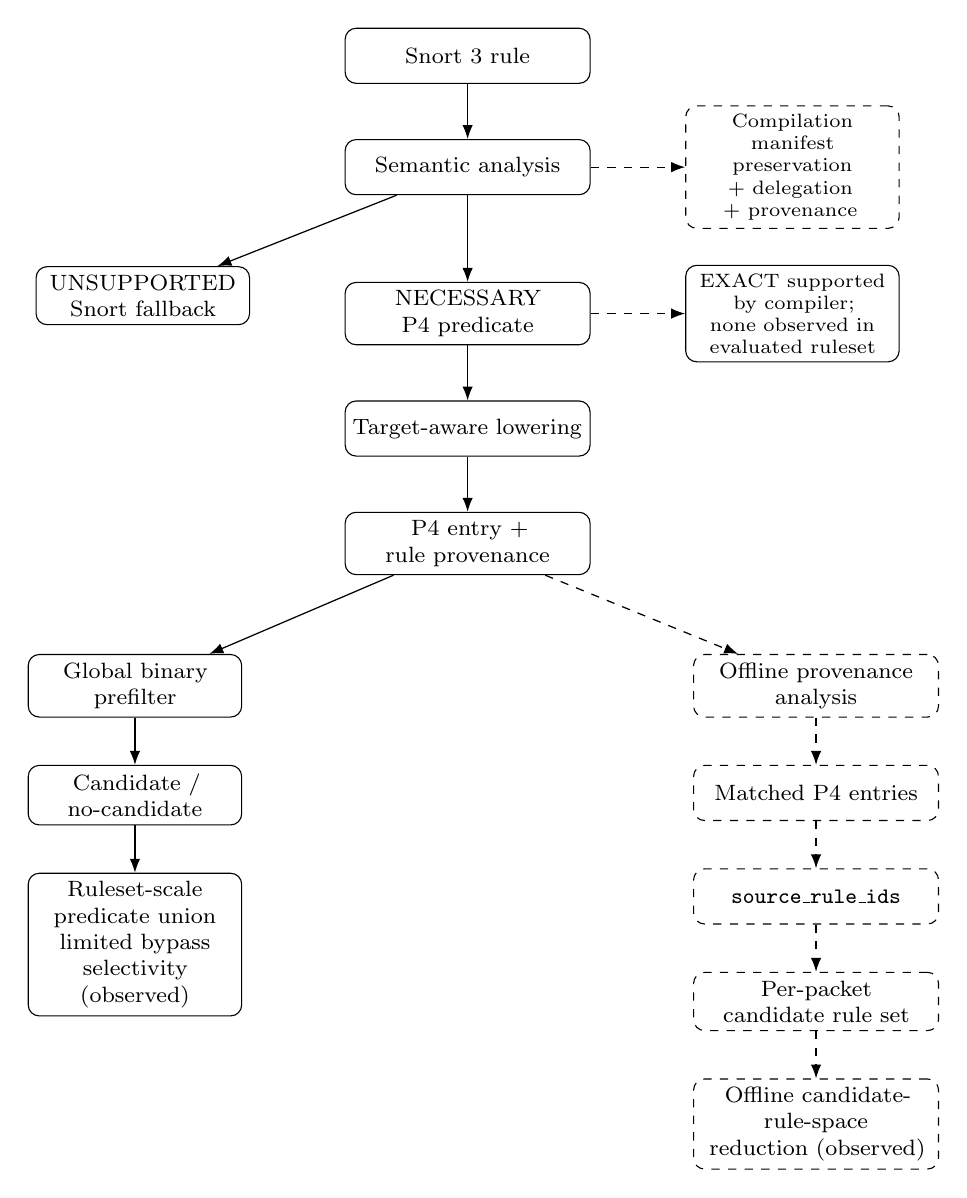
\begin{tikzpicture}[
  >=Latex,
  font=\footnotesize,
  box/.style={draw, rounded corners, align=center, minimum height=7mm,
    text width=29mm, inner sep=3pt},
  smallbox/.style={draw, rounded corners, align=center, minimum height=7mm,
    text width=25mm, inner sep=3pt},
  offline/.style={box, dashed},
  flow/.style={->, line width=.45pt},
  analysis/.style={->, dashed, line width=.45pt}
]
  \node[box] (rule) {Snort 3 rule};
  \node[box, below=7mm of rule] (semantic) {Semantic analysis};
  \node[smallbox, below left=9mm and 12mm of semantic] (fallback)
    {UNSUPPORTED\\Snort fallback};
  \node[box, below=11mm of semantic] (predicate)
    {NECESSARY\\P4 predicate};
  \node[box, below=7mm of predicate] (lowering)
    {Target-aware lowering};
  \node[box, below=7mm of lowering] (entry)
    {P4 entry +\\rule provenance};

  \node[smallbox, right=12mm of semantic, dashed, font=\scriptsize]
    (manifest) {Compilation manifest\\preservation + delegation\\+ provenance};
  \node[smallbox, right=12mm of predicate, font=\scriptsize]
    (exact) {EXACT supported by compiler;\\none observed in evaluated ruleset};

  \node[smallbox, below left=10mm and 13mm of entry] (global)
    {Global binary\\prefilter};
  \node[smallbox, below=6mm of global] (metadata)
    {Candidate /\\no-candidate};
  \node[smallbox, below=6mm of metadata] (selectivity)
    {Ruleset-scale predicate union\\limited bypass selectivity\\(observed)};

  \node[offline, below right=10mm and 13mm of entry] (provenance)
    {Offline provenance\\analysis};
  \node[offline, below=6mm of provenance] (matched)
    {Matched P4 entries};
  \node[offline, below=6mm of matched] (ids)
    {\texttt{source\_rule\_ids}};
  \node[offline, below=6mm of ids] (candidates)
    {Per-packet\\candidate rule set};
  \node[offline, below=6mm of candidates] (reduction)
    {Offline candidate-rule-space\\reduction (observed)};

  \draw[flow] (rule) -- (semantic);
  \draw[flow] (semantic) -- (fallback);
  \draw[flow] (semantic) -- (predicate);
  \draw[analysis] (semantic) -- (manifest);
  \draw[analysis] (predicate) -- (exact);
  \draw[flow] (predicate) -- (lowering);
  \draw[flow] (lowering) -- (entry);
  \draw[flow] (entry) -- (global);
  \draw[flow] (global) -- (metadata);
  \draw[flow] (metadata) -- (selectivity);
  \draw[analysis] (entry) -- (provenance);
  \draw[analysis] (provenance) -- (matched);
  \draw[analysis] (matched) -- (ids);
  \draw[analysis] (ids) -- (candidates);
  \draw[analysis] (candidates) -- (reduction);
\end{tikzpicture}
\caption{Semantics-aware, target-aware compilation overview. Semantic analysis
retains unsupported or delegated semantics in Snort while deriving necessary
P4 predicates; for service-based rules they keep only the header addresses
(Section~\ref{sec:service-based}). Target-aware lowering preserves source-rule
provenance. The implemented global binary prefilter aggregates predicates into
candidate metadata and showed limited packet-bypass selectivity in the
evaluated ruleset. The dashed provenance branch is an offline feasibility
analysis for deriving per-packet candidate rule sets; dynamic
candidate-set-aware IDS execution is not implemented. EXACT is supported by
the classifier but was not observed in the evaluated ruleset.}
\label{fig:semantic-compilation-overview}
\end{figure}

\FloatBarrier
\section{Discussion}
\subsection{Semantic Safety Does Not Imply Operational Selectivity}
For a Snort rule $r$ and a generated P4 predicate $p_r$, the relation
$r \Rightarrow p_r$ states that $p_r$ is a safe necessary condition under the
supported semantic profile and inside the enforced packet domain $D$, with
traffic outside $D$ retained through fail-open fallback. It does not
establish $p_r \Rightarrow r$ or
$r \Leftrightarrow p_r$. Semantic safety therefore asks whether traffic that
satisfies the rule also satisfies its compiled predicate; operational
selectivity asks how much other traffic that predicate can exclude.

Under the evaluated profile, 3,996 of 4,017 rules were classified as
\textsc{Necessary}, 21 as \textsc{Unsupported}, and none as \textsc{Exact}.
Nevertheless, the global binary prefilter marked 100\% of parser-eligible
packets as candidates in SQLi, XSS, and held-out Brute Force. This is not a
contradiction. The usefulness of a safely compiled predicate is not
determined solely by whether it preserves a necessary condition, but also by
how that predicate composes with predicates generated for the remainder of
the ruleset. The absence of \textsc{Exact} classifications is both a
limitation of the evaluated target/profile and evidence that partial
semantic preservation was not promoted to equivalence.
\subsection{The Union Effect in Large Rule Sets}
Conceptually, the global candidate decision is the disjunction
$P_{\mathrm{global}}(x)=p_1(x) \lor p_2(x) \lor \cdots \lor p_n(x)$.
Individual predicates may be useful filters, but the aggregate coverage of a
large disjunction can approach the workload population. The causal audit
identified broad initial contributors: \texttt{p4-88} matches TCP only,
\texttt{p4-10} matches a destination in \texttt{HOME\_NET}, and
\texttt{p4-51} matches a source in \texttt{HOME\_NET}; the last two carry the
provenance of most service-based rules.

Broad predicates were an initial contributor, but they were not a complete
explanation. The strong-discriminator ablation retained 225 entries for 739
P4-eligible rules, placed 3,257 rules in operational fallback, and retained
21 semantic \textsc{Unsupported} rules in fallback. Even then, the held-out
Brute Force trace had a 94.885\% candidate rate among parser-eligible
packets. A few retained entries are structurally specific, an ACK bit toward
\texttt{HOME\_NET} and the web and DNS ports from it, yet coincide with most
of the traffic; under the earlier compilation, the residual coverage was
instead spread across many retained predicates. Thus, the evidence does not
attribute poor selectivity to only three broad entries. It instead indicates
that large heterogeneous rulesets, together with the traffic they are written
for, can make a single global candidate bit too coarse and discard
rule-level provenance.

The union also limits what can be tested. In the end-to-end campaign, every
confirmed witness under the global plan was also matched by another rule's
entry, so a defect in any single rule's lowering would have been masked by
the rest of the table. Only after the broad entries were removed did 36
confirmations depend on the rule's own entries alone. Testing the lowering
of an individual rule therefore needs a configuration in which that rule's
predicate is not covered by the others, a condition closely related to the
one that packet-level selectivity depends on.
\subsection{From Packet Bypass to Candidate-Rule Selection}
The global prefilter asks whether a packet should remain a candidate for IDS
handling. Provenance enables a different question: which IDS rules remain
plausible candidates for that packet? The latter is obtained by mapping
matched P4 entries to their recorded source-rule IDs and taking their union
as a per-packet candidate rule set. Rule-level provenance consequently
retains information that a global candidate bit discards.

Using the 739-rule strong-discriminator baseline, the mean candidate set
contained about four rules in each trace, 4.48 on held-out Brute Force
(median 3; P99 8; maximum 293), a reduction above 99.3\% within that
partition. The partition, however, holds only the rules whose predicates the
policy treats as discriminating. The 3,278 fallback rules bound what any
candidate set can save: counted against the full ruleset, the reductions are
18.29--18.30\%, and no packet can fall below 3,278 applicable rules.

The comparison with the earlier compilation locates the loss. With the
header ports of service-based rules, the same derivation reduced the
held-out candidate set by 81.81\% over the full ruleset; without them, most
of those rules keep only an address condition on \texttt{HOME\_NET} and fall
back. Much of what header provenance appeared to discriminate was therefore
the header port, which Snort~3 does not use once it knows the service. A
candidate selector that also used the identified service, which Snort itself
uses to reject rules of other services, is a natural next step; this paper
does not evaluate one.

This observation motivates a future design space involving rule masks,
rule partitions, hierarchical selectors, candidate metadata, and
dependency-aware scheduling in hybrid P4/IDS systems. It is not evidence of
a runtime implementation: candidate-set-aware Snort execution was not
implemented, no throughput or latency benchmark was conducted, and no
speedup is demonstrated. In particular, dynamic stateful rule execution
remains unresolved.
\subsection{Why Coarse Grouping Does Not Help}
The candidate-rule-space reduction within the P4-eligible partition was
produced by fine-grained entry-to-source-rule provenance, not by grouping.
Measured directly, grouping gives back the discrimination it aggregates: a
coarse group forwards every rule it contains, and under protocol grouping,
whose TCP group holds 642 of the 739 rules, the mean reduction falls to
20--25\%. Finer groupings recover it step by step, and the two that include
the service come within half a percentage point of entry-level provenance
(Table~\ref{tab:grouped}). Over the full ruleset, the fallback rules dominate
either way.

Coarse structural groups aggregate rules whose necessary predicates remain
different. This does not show that every grouping is unhelpful: the four
evaluated strategies are structural, and the grouped set was computed
offline. Future grouping designs could account for provenance, semantic
dependencies, rule overlap, flow/state dependencies, and hardware resource
constraints.
\subsection{Implications for P4-Based IDS Offloading}
The evaluated results suggest that translation rate alone is insufficient for
assessing a P4-based IDS prefilter. Classifying 99.48\% of rules as
\textsc{Necessary} did not imply operationally selective binary packet
bypass. This complements prior work on rule-derived P4 filtering and
resource-aware data-plane representations \cite{lewis2019p4id,tavares2021p4onids}:
the semantic relation between the original rule and the compiled predicate
must remain explicit.

Semantic transparency should therefore be a first-class compiler output. A
useful artifact records preserved predicates, delegated predicates, fallback
rules, and unsupported rules rather than presenting partial translation as
full rule offload. The evidence also supports evaluation along multiple axes:
semantic coverage, target feasibility, installation state, packet-level
selectivity, observed alert preservation, and candidate-rule-space reduction.
Work on context required by rule-based prefiltering further reinforces the
need to account for IDS state beyond packet-header matching \cite{brum2025rethinking}.

The service-based case shows that even the header of a rule is not
self-describing. What a header condition means depends on how the IDS
evaluates it, and Snort~3 drops the port and protocol conditions of
service-based rules once a flow's service is known. The earlier compilation,
which derived port conditions from those headers, produced a
strong-discriminator plan that marked no-match packets on which Snort
alerted; its global plan stayed candidate-complete for all but nine of these
rules only through the broad entries that removed packet-level selectivity.
Compiled as Snort~3 evaluates them, the rules are safe under both plans, but
their predicates shrink to address conditions on \texttt{HOME\_NET} that
match most of the traffic, and the strong-discriminator policy leaves them
to fallback. Safety and selectivity pulled against each other within the
same rules.

Binary packet bypass may be too coarse for large heterogeneous rulesets under
the evaluated configuration. Predicate provenance can instead be treated as
a compiler output in its own right: it can inform downstream rule-selection
mechanisms even where a binary candidate decision is not selective. This is
an architectural implication, not an implemented acceleration or a claim
about current Snort capabilities. It is consistent with the broader interest
in coordinated programmable-data-plane and IDS processing
\cite{hagen2025rna}.

\section{Threats to Validity and Limitations}
\label{sec:threats}
\subsection{Construct Validity}
The reported metrics characterize different constructs and should not be
collapsed into a single notion of offloading effectiveness. Semantic coverage
measures whether a safe P4 predicate was derived under the supported profile;
it does not measure semantic equivalence. In particular, the 3,996
\textsc{Necessary} classifications do not constitute full Snort rule
offload, and \textsc{Exact}=0 means that no evaluated rule had all of its
semantics represented by the P4 predicate. This is both a limitation of the
evaluated target/profile and a consequence of the conservative classifier,
which does not label partial preservation as equivalence.

The \textsc{Necessary} classification itself rests on a model of Snort's
header evaluation (Section~\ref{sec:service-based}): which rules are
service-based, which header fields Snort skips for them, and that the
\texttt{flags} option matches only TCP. The model was established from the
Snort~3.12.2.0 source and documentation, and confirmed on BMv2 for one
service and one port: 190 HTTP rules alerted on port 18080, and under the
current compilation every such witness was a candidate or belonged to a rule
in fallback. An earlier compilation, which treated a service as an
additional delegated condition, over-constrained 2,931 predicates, and its
strong-discriminator plan marked all 190 witnesses no-match. A model that
missed another way in which Snort skips header conditions would fail in the
same way, and a different Snort version could change these rules; for
inspector buffers whose registration was not traced, the compiler counts the
rule as service-based, which only broadens its predicate.

Similarly, the 94.18\% backend reduction measures P4 installation state,
not traffic reduction or removal of rules from Snort. Packet-level
selectivity measures candidate rates only among parser-eligible frames,
whereas candidate-rule-space reduction is an offline feasibility metric and
not a runtime execution reduction. Observed alert preservation is empirical
and finite rather than formal equivalence. No throughput, latency, or speedup
was measured. Finally, CICIDS2017 attack-window names do not by themselves
establish the semantic meaning of the Snort alerts observed in those windows;
an SQLi, XSS, or Brute Force window should not be interpreted as evidence
that the corresponding attack class was detected unless the fired rule
semantics support that conclusion.

\subsection{Internal Validity}
SQLi and XSS were used as development and diagnostic traces, whereas Brute
Force was preserved as a held-out trace. No policy retuning was performed
after inspecting the held-out trace. The strong-discriminator configuration
is an operational ablation rather than a new semantic classification, and
its criterion and the grouping strategies were fixed before held-out
validation under the earlier compilation and applied unchanged to the
current one. Experiment artifacts were frozen, with integrity checks
recorded where applicable, and the earlier compilation's artifacts are
archived and regenerate byte for byte.

The causal analysis initially identified broad predicates, and the residual
analysis showed that coverage persisted through the entries that remained.
This reduces the risk of attributing the observed behavior only to a small
number of broad rules. It does not establish causal proof beyond the
performed ablations.

Flowbit dependency audits were performed for both partitions of the
ruleset. In the semantic partition, all 636 flowbit producer-to-consumer
edges stay inside the candidate side, so running the \textsc{Unsupported}
rules separately does not break a flowbit. The strong-discriminator
partition is not closed under flowbits: 24 edges cross it, all on one
flowbit, \texttt{smb.trans2}, between two port-based rules that remain
P4-eligible (SIDs 3143 and 3144) and ten \texttt{netbios-ssn} rules in
fallback. A deployment that ran the two sides of that partition as separate
rule sets would have to keep this flowbit component together. The absence of
other cross-partition dependencies does not establish safety for arbitrary
Snort rulesets or all stateful mechanisms.

Semantic split preservation has limited discriminating power in the evaluated
traces. The \textsc{Unsupported} partition contains 21 rules, and none of them
produced an alert in any of the three traces. The comparison of the
\textsc{Unsupported} side therefore contrasted an empty expected set with an
empty run, and the candidate side necessarily coincided with the FULL alert
set. The reported zero missing and zero additional alerts are correct, but a
partition that assigned rules incorrectly would yield the same result whenever
the misassigned rules are silent on the evaluated traffic. This measure
establishes that removing the \textsc{Unsupported} rules did not perturb the
observed alerts; it does not establish that the split is correct for rules
that the traces never exercised. Rulesets or traces that activate
\textsc{Unsupported} rules would be required to give this check
discriminating power. The end-to-end campaign does not close this gap: the 14
rules that both compilations classify as \textsc{Unsupported} admit no
synthesized witness, and the campaign does not run Snort on the two
partitions separately.

The campaign's witnesses are synthesized from the compiler's own IR, so the
generator and the compiler could share an error. The verdict does not rest on
that IR, however: a case counts only when Snort, running the original rule
text, alerts on it, so an IR error that produced a wrong witness yields a
\textsc{Vacuous} case rather than a \textsc{Confirmed} one. Vacuous cases
exposed two IR defects in \texttt{content} handling, whitespace inside the
pattern and negation written as \texttt{!} outside the quotes, and both were
corrected without changing any P4 artifact. Both runs replay the trace of the
final witness-generator revision, which preceded only the second correction;
the only sampled rule it affected, SID 28982, was recorded as vacuous. The
campaign's reach is also bounded by construction. Each rule is exercised at a
single point of its packet space, always on a port of its own header, so the
campaign cannot observe the service-based evaluation of
Section~\ref{sec:service-based}; only the dedicated off-port test does.
The 1,875 rules for which no witness can be synthesized, most of which carry
the richer payload and state semantics, are not tested at all, and the sample
is drawn from the synthesizable subset rather than from the full ruleset.

\subsection{External Validity}
These results should be interpreted within the experimental Snort variable
profile, one Community ruleset/version, and the selected CICIDS2017 Thursday
windows. The variable profile is experimental rather than an official
canonical Snort configuration. Different Community versions, custom or
private rulesets, \texttt{HOME\_NET} definitions, service-port profiles,
rule-base sizes, traffic distributions, IDS workloads, attack mixes, or
encrypted-traffic distributions may change the semantic classification,
candidate rate, and candidate rule set size. The high \textsc{Necessary}
rate, the global candidate rate, and the observed reductions should therefore
not be assumed to hold unchanged outside this configuration.
Beyond the evaluated ruleset, the compiler was exercised at compile time
only: it compiled the Snort~2.9.15.1 rules distributed by Ubuntu, both raw
and converted by \texttt{snort2lua}, once the 48 rule lines using variables
that Snort~3 does not define, and therefore also rejects, were removed. The
ten header-only rules of that ruleset are the only \textsc{Exact}
classifications observed, and they agreed with Snort on all 340 sampled
frame--rule pairs, with the P4 side evaluated by the offline matcher.

Only selected Thursday CICIDS2017 windows were evaluated for alerts. For the
packet-level quantities alone, we also measured the entire Thursday capture
offline (9,322,025 frames, 9,240,405 parser-eligible), which contains the
three windows. The global plan still marks every eligible packet as a
candidate, and the strong-discriminator plan 95.335\%. The mean candidate set
is 4.27 rules, a 99.42\% reduction within the P4-eligible partition, or
18.29\% over the full ruleset; protocol grouping reduces it by 19.68\%. The
windows are therefore not atypical of the day, but Snort alerts were not
computed for the rest of it. The dataset is old relative to current
production traffic, and its traffic mix may not reflect contemporary
enterprise networks. Held-out Brute Force strengthens the evidence within
this experimental setup, but it does not establish broad real-world
generalization to production networks, other datasets, or other IDS
workloads.

The trace-based alert evidence rests on few rules: the three windows fired
one, two, and five distinct SIDs, all of them in fallback under the
strong-discriminator plan. The end-to-end campaign widens rule coverage to
958 confirmed SIDs under the global plan and 134 under the
strong-discriminator plan, but its traffic is synthetic, one short flow per
rule, and says nothing about how often these rules fire, or which packets
they fire on, in real traffic.

\subsection{Implementation and Target Limitations}
The prototype uses the BMv2/v1model software target rather than production
ASIC hardware. It was not evaluated on production hardware, and the
evaluation does not establish deployment scalability beyond the validated
table state. No hardware timing, resource-utilization, line-rate, throughput,
or latency measurement was conducted.

The implemented parser follows the current Ethernet/IPv4 path and does not
support VLAN encapsulation. TCP, UDP, and ICMP are the principal handled L4
protocols, but the implementation does not provide generic support for every
encapsulation or protocol. Parser-ineligible frames are outside the
candidate-rate denominator rather than being P4 no-matches. Moreover, the P4
program marks candidate metadata; it does not implement a complete forwarding
or bypass architecture that safely removes Snort from the path for arbitrary
traffic.

These parser limits are handled by exclusion rather than by silent
approximation. IPv4 options, fragments, truncated headers, and parser errors
are gated out of predicate evaluation and marked candidate through domain
fallback, so the safety relation is stated over $D$ and the pipeline fails
open elsewhere. The cost is that selectivity is claimed only over $D$: a
deployment whose traffic contains substantially more options, fragments, or
tunneling than the evaluated traces would push a larger share of packets
into unconditional fallback, which is safe but less informative. Extending
the parser to cover those cases selectively, rather than conservatively,
remains future work.

Some header conditions that the target could represent are still omitted,
which only broadens their predicates: port ranges, although the port keys
are ternary and a range decomposes into prefixes; ICMP type and code; and
the protocol number given by \texttt{ip\_proto}. Representing them would
take at most 54, 123, and 3 rules out of the 3,278 that the
strong-discriminator plan applies to every packet, so it could raise that
plan's full-ruleset reduction by at most 1.3, 3.1, and 0.07 percentage
points. ICMP type and code would also need new table keys.

Replay accounting reconciles frame for frame with the data-plane counters in
all three traces under both plans, and for the alert packets replayed alone.
An earlier held-out replay, without the longer veth queues and the 2~ms
inter-frame delay, lost 87 of 1,108,658 frames (0.008\%) in the transport
layer, all within the candidate category; with them, every replay delivered
and counted every frame.

\subsection{Limitations of the Candidate-Set Analysis}
The candidate rule set analysis reported mean reductions of 99.39--99.47\%
within the P4-eligible partition and 18.29--18.30\% over the full ruleset.
These values are offline candidate-rule-space feasibility measurements, and
the traces exercise none of the retained predicates: every observed alert
belongs to a fallback rule. The current prototype does not implement dynamic
per-packet Snort rule activation, candidate-rule masks inside Snort, rule
scheduling driven by P4 metadata, a candidate-set aware Snort execution
engine, or throughput benchmarking of reduced rule sets.

Stateful semantics make dynamic execution a separate research problem. Even
when an alert SID is present in the packet's candidate set, detection can
depend on prior flow state, stream state, flowbits, temporal conditions, or
state established by previous packets. The dependency audit reduces one
specific class of risk, and it found one flowbit component that crosses the
strong-discriminator partition; it does not prove dynamic safety for all
Snort state mechanisms. The campaign measured one such mechanism directly:
Snort attributed the alerts of 606 HTTP rules to an acknowledgment that does
not satisfy the rule's header, and the strong-discriminator plan marked 445
of those acknowledgments no-match. These rules are in fallback under the
current compilation, but under the earlier one two of them were prefiltered,
so a packet-level decision that is safe for the rule's own packets can still
withhold a packet that stream inspection needs. Likewise, the grouped
candidate set was computed offline for four structural strategies only, and
it does not show that every future grouping algorithm would fail; future
evaluation should consider provenance, dependencies, overlap, and target
resource constraints together.

\section{Conclusion}
This work examined how Snort 3 detection semantics can be partially compiled
into predicates executable in a P4 data plane without obscuring semantic loss,
and whether those predicates remain useful when composed at ruleset scale. The
result is a semantics-aware, target-aware compilation workflow in which the
semantic relation of each generated predicate is explicit and predicate
provenance is retained through backend lowering.

For RQ1, all 4,017 evaluated rules were parsed; 3,996 were classified
\textsc{Necessary} and 21 remained \textsc{Unsupported}, while no rule was
\textsc{Exact}. Under the implementation assumptions of
Section~\ref{sec:problem}, the construction gives $r \Rightarrow p_r$ inside
the enforced packet domain, with options, fragments, and truncated headers
retained by fail-open fallback, and without presenting partial preservation
as equivalence. For the 2,931 service-based rules, this required compiling
only their header addresses, because Snort~3 skips header ports and protocol
once it identifies the flow's service. An earlier compilation that kept them
over-constrained those predicates, and on BMv2 its strong-discriminator plan
marked no-match the witnesses of 190 HTTP rules on which Snort alerted off
their header port. For RQ2, 4,040 source predicate instances were lowered to
235 final installation entries, a 94.18\% installation-state reduction, and
the 235-entry plan was installed and read back on the evaluated BMv2/v1model
target without encoding or validation failures.

RQ3 showed that semantic coverage and operational selectivity are distinct.
Under the evaluated configuration, the binary global prefilter marked all
parser-eligible packets as candidates in the SQLi, XSS, and held-out Brute
Force traces, replayed on BMv2 with exact accounting; the
strong-discriminator ablation still marked 92.2--94.9\%. Broad necessary
predicates contributed initially, and a few structurally specific entries
that coincide with the dominant traffic sustained the coverage after they
were removed.

For RQ4, the evaluated predicates achieved 100\% observed alert preservation
in the three traces, and the end-to-end campaign observed no violation of
$r \Rightarrow \mathrm{cand}$ among the sampled rules that Snort confirmed:
958 under the global plan and 134 under the strong-discriminator plan, 36 of
the latter attributable to the rule's own entries alone. The same campaign
showed that the global plan's broad entries leave no confirmation
attributable to a single rule, and that HTTP alerts often fall on an
acknowledgment that does not satisfy the rule's header. Provenance exposed
per-packet candidate rule sets of about four of the 739 P4-eligible rules,
but the 3,278 fallback rules apply to every packet, and the reduction over
the full ruleset is 18.29--18.30\%. Under the earlier compilation, the same
derivation reported 81.81\% on held-out Brute Force, most of it from header
ports that Snort~3 does not check. This candidate-set result is an offline
feasibility result, not a dynamic IDS execution result. The central
implication is that semantic correctness and operational usefulness are
distinct dimensions of IDS rule offloading, and that a prefilter's apparent
selectivity has to be checked against how the IDS evaluates each rule.
Future work should implement candidate-set-aware and dependency-aware IDS
execution, investigate selectors that use the identified service as well as
header provenance, then evaluate execution cost on hardware targets and
broader rulesets, profiles, traffic datasets, and parser/protocol/
encapsulation coverage.

\section*{Artifact Availability}
The compiler, the experimental variable profile, the analysis scripts, and the
frozen output artifacts reported in this paper are available at
\url{https://github.com/medeiros08/Snort-p4}. The repository contains the
compilation pipeline from rule parsing to P4Runtime entry generation, the
semantic manifest with predicate-to-rule provenance, the compiled P4 program
and its P4Info, and the JSON artifacts underlying every table and figure. A
regression check reproduces the ten pipeline artifacts byte for byte from the
committed sources; the earlier compilation's artifacts are archived and
regenerate byte for byte from the same sources with its header semantics
selected. The end-to-end campaign's cases, per-case verdicts, and Snort
alerts are under \path{output/campaign/}; its traces are not versioned, but
the case generator at the commit that produced a run should regenerate its
trace byte for byte; this was checked against the SHA-256 digest recorded
with the run.

The CICIDS2017 traces are not redistributed here; they are obtained from the
Canadian Institute for Cybersecurity. The BMv2 target, Snort~3, and the P4
compiler are third-party software and are not redistributed; the exact
versions used to produce the frozen artifacts are stated in
Section~\ref{sec:methodology}, and \path{scripts/setup_bmv2.sh} reproduces the
data-plane configuration they ran under.

\appendix
\section{Experimental Snort Variable Profile}
\label{app:snort-profile}
The evaluated CICIDS2017 configuration used the \texttt{cicids2017} profile
from \path{config/profiles/cicids2017.json}. Its resolved variables were
written to \path{config/snort_variables.json}. The generated Snort
configuration is \path{config/snort3_experiment.lua}; the active-profile
record identifies the same profile. Table~\ref{tab:snort-profile} documents
the resulting variables used for the 4,017-rule evaluation.

\begin{table*}[t]
\centering
\small
\caption{Experimental Snort variable profile used for the CICIDS2017
evaluation.}
\label{tab:snort-profile}
\begin{tabular}{lll}
\toprule
\textbf{Variable} & \textbf{Experimental value} & \textbf{Role} \\
\midrule
\texttt{HOME\_NET} & \texttt{192.168.10.0/24} & protected network \\
\texttt{EXTERNAL\_NET} & \texttt{any} & external network \\
\texttt{HTTP\_SERVERS} & \texttt{192.168.10.0/24} & HTTP server scope \\
\texttt{SQL\_SERVERS} & \texttt{192.168.10.0/24} & SQL server scope \\
\texttt{SMTP\_SERVERS} & \texttt{192.168.10.0/24} & SMTP server scope \\
\texttt{TELNET\_SERVERS} & \texttt{192.168.10.0/24} & TELNET server scope \\
\texttt{SIP\_SERVERS} & \texttt{192.168.10.0/24} & SIP server scope \\
\texttt{HTTP\_PORTS} & \texttt{80 8080} & HTTP service ports \\
\texttt{ORACLE\_PORTS} & \texttt{1521} & Oracle service ports \\
\texttt{FILE\_DATA\_PORTS} & \texttt{80 110 143} & file-data service ports \\
\texttt{SIP\_PORTS} & \texttt{5060 5061} & SIP service ports \\
\texttt{SSH\_PORTS} & \texttt{22} & SSH service ports \\
\texttt{FTP\_PORTS} & \texttt{21} & FTP service ports \\
\bottomrule
\end{tabular}
\end{table*}

The generated configuration includes the standard Snort configuration and
then explicitly disables the default inclusion of
\texttt{file\_magic.rules} by setting \verb|file_inspect = {}|.
Consequently, the evaluated ruleset contains only the intended 4,017
community rules.

This is an experimental variable profile, not an official canonical Snort
configuration. The semantic classifications and selectivity measurements are
configuration dependent: changing network variables or service-port
definitions can change the generated necessary predicates and their
selectivity. This profile-specific scope is considered in the threats to
validity discussion.
\bibliographystyle{plain}
\bibliography{references}

\end{document}
